% !Mode:: "TeX:UTF-8"
%% 请使用 XeLaTeX 编译本文.
\documentclass[forprint, AutoFakeBold, AutoFakeSlant ]{WHUExperiment}
%---------------------这里添加所需的命令--------------------------------
\lstdefinelanguage{json}{ % 定义json代码高亮
    morestring=[d]",
    stringstyle=\color{red!50!brown},
    showstringspaces=false,
    literate=
     *{0}{{{\color{Gray}0}}}{1}
      {1}{{{\color{Gray}1}}}{1}
      {2}{{{\color{Gray}2}}}{1}
      {3}{{{\color{Gray}3}}}{1}
      {4}{{{\color{Gray}4}}}{1}
      {5}{{{\color{Gray}5}}}{1}
      {6}{{{\color{Gray}6}}}{1}
      {7}{{{\color{Gray}7}}}{1}
      {8}{{{\color{Gray}8}}}{1}
      {9}{{{\color{Gray}9}}}{1}
      {:}{{{\color{Purple}{:}}}}{1}
      {,}{{{\color{Purple}{,}}}}{1}
      {\{}{{{\color{BlueGreen}{\{}}}}{1}
      {\}}{{{\color{BlueGreen}{\}}}}}{1}
      {[}{{{\color{BlueGreen}{[}}}}{1}
      {]}{{{\color{BlueGreen}{]}}}}{1},
}

%--------------------------------------------------------------------------
\makeatletter
\def\BState{\State\hskip-\ALG@thistlm}
\makeatother
\begin{document}
%-----------------------------------------------------------------------------

%%%%%%% 下面的内容, 据实填空.

\Ccoursename{XXX课程} %课程名称
\title{ ~\LaTeX~ 模板及使用教程\\Introduction of ~\LaTeX~ Template} %实验名称 换行请使用\\
\author{} % 学生姓名
\Csupervisor{XXXX \quad 教授} %指导教师一姓名、职称

% 默认不显示指导教师二,需要时可在WHUExperiment.cls 80+行处将"关闭第二指导教师显示"下一行的注释解除
\CsupervisorAnother{无} %指导教师二姓名、职称 

\CstudentNum{XXXX} %学号
\Cmajor{XXXX} % 专业名称
\date{二〇二二年七月} % 日期

%-----------------------------------------------------------------------------

\pdfbookmark[0]{封面}{title}         % 封面页加到 pdf 书签
\maketitle
\frontmatter
\pagenumbering{Roman}              % 正文之前的页码用大写罗马字母编号.2019.6.16:更新 正文之前的页码隐藏,无需显示
%-----------------------------------------------------------------------------
% !Mode:: "TeX:UTF-8"

%%% 此部分需要自行填写: 中文摘要及关键词 

%%% 郑重声明部分无需改动

%%%---- 郑重声明 (无需改动)------------------------------------%
\newpage
\thispagestyle{empty}
\vspace*{20pt}
\begin{center}{\ziju{0.8}\pmb{\songti\zihao{2} 郑重声明}}\end{center}
\par\vspace*{30pt}
\renewcommand{\baselinestretch}{2}

{\zihao{4}%

本人呈交的设计报告,是在指导老师的指导下,独立进行实验工作所取得的成果,
所有数据、图片资料真实可靠。 尽我所知,除文中已经注明引用的内容外,
本设计报告不包含他人享有著作权的内容。
对本设计报告做出贡献的其他个人和集体,
均已在文中以明确的方式标明。本设计报告的知识产权归属于培养单位。\\[2cm]

\hspace*{1cm}本人签名: $\underline{\hspace{3.5cm}}$
\hspace{2cm}日期: $\underline{\hspace{3.5cm}}$\hfill\par}
%------------------------------------------------------------------------------
\baselineskip=23pt  % 正文行距为 23 磅
%------------------------------------------------------------------------------





%%======摘要===========================%
\begin{cnabstract}
\thispagestyle{empty}
本实验旨在研究基于云原生微服务架构的 web 商城应用 Online Boutique,并将其部署在 Kubernetes 环境中。通过实验,我深入研究了微服务架构、服务治理和监控方面的相关技术,并应用于 Online Boutique 项目中。

首先,本实验安装了 Kubernetes 集群环境,并通过部署 Dashboard 实现了集群中的可视化管理。我们探讨了不同安装方式,包括二进制安装、kubeadm 安装、minikube 和 kubesphere,并选择适合需求的安装方式。随后,本实验成功将基于微服务架构的 Online Boutique 应用部署在 Kubernetes 环境中,并验证了应用的正常运行。通过部署的过程,我们了解了如何处理微服务的部署、扩展和管理。为了解决 Online Boutique 在熔断、限流、监控、认证、授权、安全和负载等方面的不足,本实验将其升级到服务网格架构,并启用 Istio 来支持微服务。通过 Istio实现了服务拓扑发现、全链路跟踪、指标遥测和健康检查等功能,实现了更强大的服务治理。

在进一步提升可观测性方面,配置了 Kiali 和 Jaeger,为 Online Boutique 项目提供了服务网格的可视化和分布式调用链追踪系统,能够监控和排查基于微服务的分布式系统问题,并进行根因分析和性能优化。安装和配置了 Prometheus 和 Grafana,实现了对整个 Kubernetes 集群和工作负载的运行情况和健康状态的监控。

最后,本实验尝试将 Online Boutique 项目中的一个非 Java 实现的微服务改写成 Spring Boot 的微服务,并重新使用之前配置的组件进行部署、调试、分析和管理。

本实验报告记录了各项实验过程,总结了各项技术平台的底层实现机制,并提供了在 Online Boutique 项目中的配置和使用步骤。通过该实验,我获得了丰富的实践经验,为今后的云原生微服务架构设计和应用提供了宝贵的参考和指导。

\end{cnabstract}
\par
\vspace*{2em}


%%%%--  关键词 -----------------------------------------%%%%%%%%
%%%%-- 注意: 每个关键词之间用“;”分开,最后一个关键词不打标点符号
\cnkeywords{云原生微服务架构;服务网格;Kubernetes}



    % 加入摘要, 申明.
%==========================把目录加入到书签==============================%%%%%%


\tableofcontents
\thispagestyle{empty}				%不显示罗马数字 ——zmx更新于2019.06.18
\addtocontents{toc}{\protect\thispagestyle{empty}}




\mainmatter %% 以下是正文
%%%%%%%%%%%%%%%%%%%%%%%%%%%--------main matter-------%%%%%%%%%%%%%%%%%%%%%%%%%%%%%%%%%%%%
\pagestyle{plain}%plain
%\cfoot{\thepage{\zihao{5}\bf\usefonttimes}}
%\renewcommand{\baselinestretch}{1.6}
%\setlength{\baselineskip}{23pt}
\baselineskip=23pt  % 正文行距为 23 磅

%此处书写正文-------------------------------------------------------------------------------------

\chapter{概述}

\section{选题背景与实验目的}
随着云计算和容器化技术的快速发展,云原生微服务架构已经成为构建现代应用程序的首选方法。微服务架构通过将应用程序拆分为小型、自治的服务,使得团队可以独立开发、部署和扩展各个服务,从而提高开发效率和应用的弹性和可伸缩性。

在微服务架构中,Kubernetes作为一个成熟的容器编排和管理平台,提供了强大的功能和工具,用于自动化应用程序的部署、弹性伸缩、负载均衡和故障恢复等方面。Kubernetes提供了一个统一的平台,简化了应用程序在分布式环境中的部署和管理,使得开发者可以专注于业务逻辑的开发,而不必过多关注底层基础设施的细节。

Online Boutique是一个由Google开发的示例应用程序,旨在演示云原生微服务架构的最佳实践。该应用程序由一组独立运行的微服务组成,模拟了一个电子商务平台,涵盖了用户界面、产品目录、购物车、订单处理等核心功能。通过研究和部署Online Boutique应用,我们可以深入了解微服务架构的实际应用场景,理解微服务之间的通信和协作方式,以及如何在Kubernetes环境中进行部署和管理。

然而,微服务架构也面临着一些挑战,例如熔断、限流、监控、认证、授权、安全和负载等方面的问题。为了解决这些挑战,引入服务网格的概念成为一种解决方案。服务网格框架Istio作为一个开源工具提供了流量管理、安全性、可观测性和策略执行等功能,为微服务架构带来更强大的服务治理能力。

因此,通过研究基于云原生微服务架构的Online Boutique应用,并将其部署在Kubernetes环境中,我们可以全面理解微服务架构、Kubernetes和服务网格技术的应用和实践。这将为我们提升云原生架构设计和实施的能力,使我们在开发和部署现代应用程序时具备更高的技术水平和竞争优势。

本实验的主要目的是:

\begin{itemize}
	\item 研究基于云原生微服务架构的Online Boutique应用,并将其部署在Kubernetes环境中。通过实际部署和运行Online Boutique应用,掌握在Kubernetes中部署和管理微服务应用的技术和方法。
	\item 探索微服务架构中存在的挑战,如熔断、限流、监控、认证、授权、安全和负载等问题,并引入服务网格的概念来解决这些挑战。通过引入Istio作为服务网格框架,实现对微服务的流量管理、安全性和可观测性的增强。
	\item 实践服务拓扑发现、全链路追踪、指标遥测、健康检查等服务治理功能,以实现对Online Boutique应用的全面监控和管理。
	\item 进一步探索在Kubernetes中配置和使用Kiali、Jaeger、Prometheus和Grafana等工具,实现服务网格的可视化、链路追踪、日志监控和健康状态监测。
\end{itemize}

通过完成以上实验目标,我将能够全面了解云原生微服务架构、Kubernetes和服务网格的应用和实践。这将为我提供宝贵的经验,使我们能够更好地设计和实施云原生架构,提升应用程序的可靠性、弹性和可伸缩性,并为开发和部署现代应用程序提供技术上的竞争优势。

\section{实验内容}

本实验将围绕着云原生微服务架构和Kubernetes展开,通过研究和实践基于云原生微服务架构的Online Boutique应用,深入探讨在Kubernetes环境中部署和管理微服务应用的最佳实践。实验将了解微服务架构的设计原则、服务拓扑发现、全链路追踪、指标遥测等关键概念,并将引入Istio作为服务网格框架,以进一步提升微服务的弹性、可观测性和安全性。

总体上,本实验的主要内容可以概括为以下几点:

\begin{enumerate}
	\item 安装和配置Kubernetes集群环境,包括安装Kubernetes和部署Dashboard,以可视化管理集群中的Pod、Service和Deployment。
	\item 将基于云原生微服务架构的Online Boutique应用部署在Kubernetes环境中,确保应用能够成功访问并展示首页。
	\item 使用Istio服务网格框架升级Online Boutique应用,以增强微服务的熔断、限流、监控、认证、授权、安全和负载等方面的能力。实现服务拓扑发现、全链路跟踪、指标遥测和健康检查等服务治理功能。
	\item 在Kubernetes中配置Kiali,实现Istio服务网格的可视化,为Online Boutique项目提供服务拓扑图、全链路跟踪、指标遥测、配置校验和健康检查等功能。
	\item 在Kubernetes中配置Jaeger,为Online Boutique项目提供分布式调用链追踪系统,监控和排查基于微服务的分布式系统问题,如分布式上下文传播、分布式事务监控、根因分析、服务依赖关系分析和性能/延迟优化。
	\item 安装和配置Prometheus、Grafana,实现对整个Kubernetes集群和工作负载的运行情况和健康状态的监控。
	\item 将Online Boutique项目中的非Java微服务改写为Spring Boot微服务,并重新部署到Kubernetes中,利用之前配置的组件进行调试、分析和管理。
	\item 总结和整理各项技术平台的底层实现机制,并提供Online Boutique项目的配置和使用步骤,以便更好地理解和应用这些技术。
\end{enumerate}

\chapter{微服务部署与验证}
\section{Kubernetes环境搭建}
为了成功部署和管理云原生微服务应用,我们需要建立一个可靠的Kubernetes集群环境。本节将简要介绍Kubernetes环境搭建的步骤,并提供系统参数配置示例。

参考本实验所使用的Kubernetes集群环境如下表所示:

\begin{table}[ht]\centering
\begin{tabular}{l|l|l}
	\hline\hline
	虚拟机hostname        & IP地址&含义              \\ \hline
	master&192.168.210.128&Kubernetes集群主节点,应用部署端,服务监控端 \\ \hline
	node1&192.168.210.129& Kubernetes集群从节点1\\ \hline
	node2&192.168.210.130& Kubernetes集群从节点2\\ 
\hline\hline
\end{tabular}
\end{table}
\subsection{虚拟机节点准备}
在开始搭建Kubernetes集群之前,确保所有虚拟客户机满足Kubernetes的最低硬件要求,并选择适合的操作系统版本。本实验使用稳定的Linux发行版CentOS 7.9,每台机器 8 GB 内存,2核4个CPU,集群中的所有机器的网络彼此均能相互连接,节点中无有重复的主机名、MAC 地址或 product\_uuid。对集群中的每台虚拟机,执行如下指令,关闭 SELinux、关闭防火墙、关闭swap分区:
\begin{lstlisting}[language=bash]
systemctl stop firewalld
systemctl disable firewalld
vim /etc/selinux/config
setenforce 0
swapoff -a
vim /etc/fstab
#注释swap
\end{lstlisting}
添加域名映射,测速节点之间是否能互相Ping:
\begin{lstlisting}[language=bash]
vim /etc/hosts
192.168.210.128 master
192.168.210.129 node1
192.168.210.130 node2
\end{lstlisting}
同步网络时间后,为三台虚拟机都添加阿里源,以绕过翻墙或下载速度过慢。
\begin{lstlisting}[language=bash]
cat <<EOF > /etc/yum.repos.d/kubernetes.repo
[kubernetes]
name=Kubernetes
baseurl=http://mirrors.aliyun.com/kubernetes/yum/repos/kubernetes-el7-x86_64
enabled=1
gpgcheck=1
repo_gpgcheck=0
gpgkey=http://mirrors.aliyun.com/kubernetes/yum/doc/yum-key.gpg http://mirrors.aliyun.com/kubernetes/yum/doc/rpm-package-key.gpg
EOF
\end{lstlisting}
为了正确配置系统参数,创建并编辑文件\texttt{/etc/sysctl.d/k8s.conf},将以下内容添加到文件中:
\begin{lstlisting}[language=bash]
net.bridge.bridge-nf-call-ip6tables=1
net.bridge.bridge-nf-call-iptables=1
net.ipv4.ip_forward=1
vm.swappiness=0
\end{lstlisting}

然后,通过运行命令\texttt{sysctl --system}使参数生效。

\subsection{为所有节点安装Docker}
Kubernetes使用Docker容器来运行应用程序。在所有节点上安装Docker,并根据实际需求进行配置。首选,添加docker的yum源:

\begin{lstlisting}[language=bash]
yum-config-manager --add-repo https://download.docker.com/linux/centos/docker-ce.repo
yum -y install docker-ce-20.10.9 docker-ce-cli-20.10.9 containerd.io
systemctl enable docker
systemctl start docker
\end{lstlisting}
接下来,编辑文件\texttt{/etc/docker/daemon.json},将以下内容添加到文件中:
\begin{lstlisting}[language=bash]
{
"registry-mirrors": ["https://b9pmyelo.mirror.aliyuncs.com"],
"exec-opts": ["native.cgroupdriver=systemd"]
}
\end{lstlisting}

此处,需要注意的是对\texttt{exec-opt}的修改:参考\citep{systemd},cgroups(Control Groups) 是 linux 内核提供的一种机制,它可以限制、记录任务组所使用的物理资源,是内核附加在程序上的hook,使程序运行时对资源的调度触发相应的钩子,达到资源追踪和限制资源使用的目的。Kubernetes 推荐使用 systemd 来代替 cgroupfs,因为systemd是Kubernetes自带的cgroup管理器, 负责为每个进程分配cgroups, 但docker的cgroup driver默认是cgroupfs,这样就同时运行有两个cgroup控制管理器, 当资源有压力的情况时,有可能出现不稳定的情况。最后,通过运行命令\texttt{systemctl restart docker}使配置生效。


\subsection{为所有节点安装Kubernetes}
首先,创建并编辑文件\texttt{/etc/yum.repos.d/kubernetes.repo},将以下内容添加到文件中:
\begin{lstlisting}[language=bash]
[kubernetes]
name = Kubernetes
baseurl = https://mirrors.aliyun.com/kubernetes/yum/repos/kubernetes-el7-x86_64
enabled = 1
gpgcheck = 0
repo_gpgcheck = 0
gpgkey = https://mirrors.aliyun.com/kubernetes/yum/doc/yum-key.gpg
https://mirrors.aliyun.com/kubernetes/yum/doc/rpm-package-key.gpg
\end{lstlisting}

然后,运行以下命令安装Kubernetes组件:
\begin{lstlisting}[language=bash]
yum -y install kubelet-1.22.6 kubeadm-1.22.6 kubectl-1.22.6
systemctl enable kubelet
\end{lstlisting}

\subsection{集群master节点初始化与node节点加入}
使用以下命令初始化Kubernetes集群:
\begin{lstlisting}[language=bash]
kubeadm init \
--apiserver-advertise-address=192.168.210.128 \
--image-repository registry.aliyuncs.com/google_containers \
--kubernetes-version v1.22.6 \
--service-cidr=10.96.0.0/12 \
--pod-network-cidr=10.244.0.0/16
\end{lstlisting}

在初始化完成后,创建存储Kubernetes配置文件的目录,然后,将管理员配置文件复制到用户目录,并设置正确的权限:
\begin{lstlisting}[language=bash]
mkdir -p $HOME/.kube
sudo cp -i /etc/kubernetes/admin.conf $HOME/.kube/config
sudo chown $(id -u):$(id -g) $HOME/.kube/config
\end{lstlisting}

使用以下命令将节点加入Kubernetes集群:
\begin{verbatim}
kubeadm join 192.168.210.128:6443 --token s19psv.t5r2ms4sos28duxc \
--discovery-token-ca-cert-hash sha256:21d529dc1ac201206aa4c0a417982bbd9561ad06e2ee34302205c51a482b7bb4
\end{verbatim}
通过执行上述命令,将节点成功加入到Kubernetes集群中。

\subsection{网络配置}
为Kubernetes集群配置网络,确保各个节点之间可以通信,并提供外部访问服务的能力。本实验采取falnnel网络插件,使用离线安装:
\begin{lstlisting}[language=bash]
kubectl apply -f kube-flannel.yml
\end{lstlisting}

\subsection{Kubernetes集群配置结果}
节点成功加入Kubernetes集群的标志是通过执行以下命令后,在输出中看到类似以下信息:
\begin{verbatim}
This node has joined the cluster:
* Certificate signing request was sent to apiserver and a response was received.
* The Kubelet was informed of the new secure connection details.
\end{verbatim}

执行 \texttt{kubectl get nodes} 命令,检查新加入的节点是否以 Ready 状态显示。
\begin{figure}[htb]
\centering
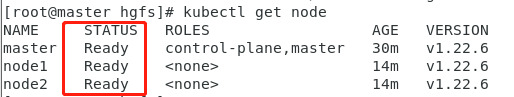
\includegraphics[width=1.0\textwidth]{figures/chapter2/getnode.png}
\caption{Kubernetes集群搭建成功后节点状态}
\label{fig:Kubernetes集群搭建成功后节点状态}
\end{figure}
至此Kubernetes集群环境搭建完毕,master作为master节点,node1,node2作为worker节点。
\begin{table}[ht]\centering
\begin{tabular}{l|l|l|l}
	\hline\hline
	服务器& 操作系统版本&	CPU架构&	功能描述\\ \hline
	master/192.168.210.128&CentOS Linux7.9&	x86\_64&k8s master节点 \\ \hline
	node1/192.168.210.129& CentOS Linux7.9&x86\_64&k8s worker节点\\ \hline
	node2/192.168.210.130& CentOS Linux7.9&x86\_64&k8s worker节点\\ 
	\hline\hline
\end{tabular}
\caption{Kubernetes集群架构}
\end{table}
\section{Kubernetes Dashboard部署}
Dashboard是一个Kubernetes集群的可视化管理工具,可以通过Web界面直观地查看和管理集群中的资源。根据兼容性要求,确认所使用的Dashboard版本与Kubernetes版本匹配。可以参考兼容性参考文档:\url{https://github.com/kubernetes/dashboard}。本实验分如下步骤搭建Dashboard环境:
使用下载好的kubernetes-dashboard-v2.0.3.yml配置文件进行安装,修改YAML文件,将Service的类型(type)修改为NodePort,并将端口(port)设置为31260。在文件的40行和44行进行修改。用kubectl命令apply -f即可。
\begin{lstlisting}[language=bash]
kubectl apply -f kubernetes-dashboard-v2.0.3.yml
\end{lstlisting}
使用以下命令验证Dashboard的Pod状态是否为Running:
\begin{lstlisting}[language=bash][language=bash]
kubectl get pod --namespace=kubernetes-dashboard -o wide | grep dashboard
\end{lstlisting}
创建Dashboard的访问权限:
\begin{lstlisting}[language=bash]
kubectl apply -f create-admin.yaml
\end{lstlisting}
其中,\texttt{create-admin.yaml}是一个包含访问权限配置的YAML文件.
获取Dashboard的访问地址:
\begin{lstlisting}[language=bash]
kubectl -n kubernetes-dashboard describe service kubernetes-dashboard
\end{lstlisting}
在输出中,找到 \texttt{LoadBalancer Ingress} 字段下的IP地址和端口号,即可访问Dashboard的Web界面。
查看Dashboard的服务端口,可以使用以下命令:
\begin{lstlisting}[language=bash]
kubectl get service -n kube-system | grep dashboard
\end{lstlisting}
确认端口号为30001。
打开Web浏览器,输入访问地址,在登录界面中选择"Token"认证方式,并将上一步中获取到的Token粘贴到相应的输入框中。并使用之前设置的访问权限进行登录。
\begin{figure}[htb]
\centering
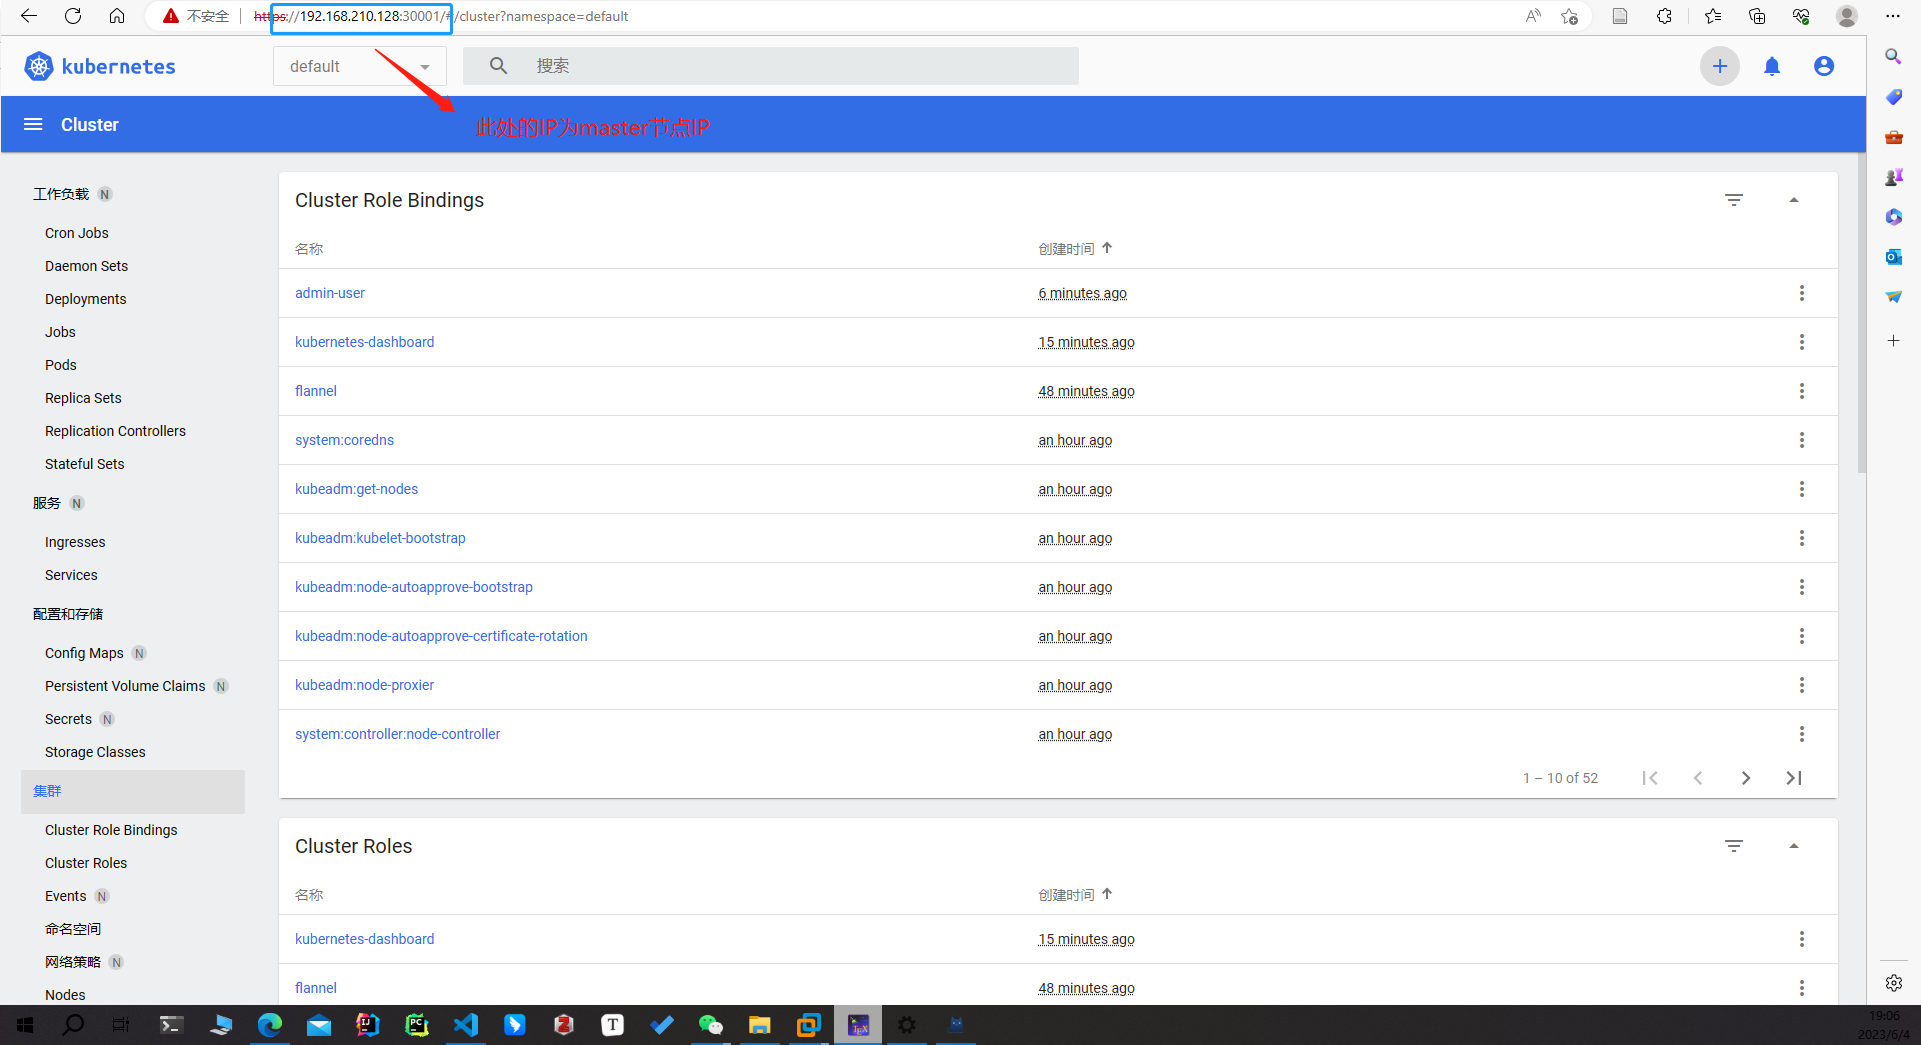
\includegraphics[width=1.0\textwidth]{figures/chapter2/dashboard.png}
\caption{Kubernetes Dashboard登录后的集群展示界面}
\label{fig2:Kubernetes Dashboard登录后的集群展示界面}
\end{figure}

\section{Istio与Online-Boutique项目微服务部署}
\subsection{单体架构与微服务架构}
在软件设计中,经常提及和使用经典的3层模型,即表示层、业务逻辑层和数据访问层。
\begin{itemize}
	\item 表示层:用于直接和用户交互,也称为交互层,通常是网页、UI 等。
	
	\item 业务逻辑层:即业务逻辑处理层,例如用户输入的信息要经过业务逻辑层的处理后,才能展现给用户。
	
	\item 数据访问层:用于操作数据库,用户在表示层会产生大量的数据,通过数据访问层对数据库进行读写操作。
\end{itemize}

虽然在软件设计中划分了经典的3层模型,但是对业务场景没有划分。一个典型的单体应用就是将所有的业务场景的表示层、业务逻辑层和数据访问层放在一个工程中,最终经过编译、打包,部署在一台服务器上。

单体架构部署简单,可以直接部署在一个服务器上即可。使用技术单一,项目不需要复杂的技术栈,往往一套熟悉的技术栈就可以完成开发,而且用人成本低 单个程序员可以完成业务接口到数据库的整个流程。但是也有一定缺陷,例如:
\begin{itemize}
	\item 系统启动慢 , 一个进程包含了所有的业务逻辑,涉及到的启动模块过多,导致系统的启动、重启时间周期过长
	
	\item 系统错误隔离性差、可用性差,任何一个模块的错误均可能造成整个系统的宕机
	
	\item 可伸缩性差;系统的扩容只能只对这个应用进行扩容,不能做到对某个功能点进行扩容
	
	\item 线上问题修复周期长;任何一个线上问题修复需要对整个应用系统进行全面升级
\end{itemize}

微服务架构风格\cite{weifuwujiagou}是一种将一个单一应用程序开发为一组小型服务的方法每一个服务运行在自己的进程中服务间通信采用的轻量级通信机制通(常用HTTP 资源 API ). 这些服务围绕业务能力构建并且可通过全自动部署机制独立部署这些服务公用一个最小型的集中式的管理服务可用不同的语言开发,使用不同的数据存储技术。

微服务架构以其易于开发和维护的特性受到广泛关注。每个微服务专注于特定的业务功能,使得业务清晰,代码量少。开发和维护单个微服务相对简单,而整个应用由多个微服务构建,使整体应用保持可控状态。此外,微服务的启动速度快,因为每个微服务的代码量较少。相比于单体架构模式,微服务解决了整个应用修改后重新部署的问题。一般情况下,对某个微服务进行修改只需要重新部署该服务即可。

在微服务架构中,可以根据项目业务和团队特点,灵活选择技术栈。不同的微服务可以使用适合的技术工具,例如关系型数据库MySQL或非关系型数据库Redis。此外,根据需求,部分微服务可以使用Java开发,而其他微服务则可以选择Node.js开发。这种灵活性使得微服务架构更加适应各种项目需求。

另外,微服务架构支持按需收缩,实现细粒度的扩展。例如,当某个微服务遇到瓶颈时,可以根据该微服务的业务特点,增加内存、升级CPU或增加节点等方式进行扩展,以满足系统的需求。

通过微服务架构,我们可以充分利用其优势,使得开发和维护变得简单高效。同时,根据项目需求和团队特点,选择适合的技术工具和灵活扩展方式,为应用提供高度可定制的解决方案。

\subsection{Online Boutique 代码分析}
Online Boutique由11个使用不同编程语言编写的微服务组成,它们通过gRPC进行相互通信。在./protos目录下可以找到协议缓冲描述。具体地,Online Boutique 由以下微服务组成:

\begin{tabularx}{\textwidth}{|l|l|X|}
	\hline
	\textbf{服务} & \textbf{编程语言} & \textbf{描述} \\
	\hline
	前端服务 & Go & 提供一个HTTP服务器来提供网站。无需注册/登录,自动生成所有用户的会话ID。 \\\hline
	购物车服务 & C\# & 将用户的购物车项目存储在Redis中并检索它。 \\\hline
	产品目录服务 & Go & 从JSON文件中提供产品列表,并能够搜索产品和获取单个产品的详细信息。 \\\hline
	货币转换服务 & Node.js & 将一个货币金额转换为另一种货币。使用从欧洲央行获取的实时数据。这是最高请求量的服务。 \\\hline
	支付服务 & Node.js & 使用给定的信用卡信息(模拟)对给定金额进行扣款,并返回交易ID。 \\\hline
	配送服务 & Go & 根据购物车提供运费估算,并将商品运送到指定地址(模拟)。 \\\hline
	邮件服务 & Python & 向用户发送订单确认邮件(模拟)。 \\\hline
	结账服务 & Go & 检索用户的购物车,准备订单,并协调支付、配送和邮件通知。 \\\hline
	推荐服务 & Python & 基于购物车内容推荐其他产品。 \\\hline
	广告服务 & Java & 根据给定的上下文词汇提供文本广告。 \\\hline
	负载生成器 & Python/Locust & 使用Locust负载生成器模拟真实用户的购物流程连续发送请求给前端。 \\
	\hline
\end{tabularx}
该项目具有以下特征:
\begin{itemize}
	\item Kubernetes/GKE:该应用程序设计为在Kubernetes上运行(包括本地的“Docker for Desktop”和云端的GKE)。
	\item gRPC:微服务之间使用大量的gRPC调用进行通信。
	\item Istio:应用程序在Istio服务网格上运行。
	\item Cloud Operations(Stackdriver):许多服务都使用了性能分析和跟踪功能。此外,使用Istio还可以获得请求/响应指标和上下文图等功能。当应用程序在Google Cloud之外运行时,这些代码路径将处于非活动状态。
	\item Skaffold:使用Skaffold命令将应用程序一键部署到Kubernetes。
	\item 合成负载生成:该应用程序演示了使用Locust负载生成器创建真实使用模式的背景作业。
\end{itemize}
\subsection{安装Istio}
本实验采用的 Istio 的版本为 1.5.7,首先检查集群是否正常。

\begin{lstlisting}[language=bash]
[root@master ~]# kubectl get node
NAME         STATUS   ROLES                  AGE    VERSION
master   Ready    control-plane,master   288d   v1.21.9
node1   Ready    <none>                 288d   v1.21.9
node2   Ready    <none>                 288d   v1.21.9
\end{lstlisting}

本实验安装 Istio 的 demo 配置文件,因为它包含所有的核心组件,并启用了跟踪和日志记录,便于学习不同的 Istio 功能,该过程主要参考博客\cite{istio},但后来部署项目时发现问题,主要是Gateway与HTTPRouter两个kind的问题,于是参考Stackoverflow中的回答\footnote{\url{https://stackoverflow.com/questions/69461513/no-matches-for-kindgateway-and-virtualservice}},下载了crd-all.gen.yaml并执行安装。

\begin{lstlisting}[language=bash][language=bash]
# 下载 GetMesh CLI
curl -sL https://istio.tetratelabs.io/getmesh/install.sh | bash

# 安装 Istio
getmesh istioctl install --set profile=demo
kubectl apply -f ./crd-all.gen.yaml
\end{lstlisting}
\subsection{Online Boutique 应用部署}
Istio 安装完成后,创建一个名为 \texttt{online-boutique} 的命名空间,新的项目将部署在该命名空间下,并为命名空间设置 \texttt{istio-injection=enabled} 标签,以启用 Sidecar 自动注入。

\begin{lstlisting}[language=bash][language=bash]
# 创建命名空间 online-boutique
[root@master ~]# kubectl create ns online-boutique
namespace/online-boutique created

# 切换命名空间
[root@master ~]# kubens online-boutique
Context "kubernetes-admin@kubernetes" modified.
Active namespace is "online-boutique".

# 让命名空间 online-boutique 启用 Sidecar 自动注入
[root@master ~]# kubectl label ns online-boutique istio-injection=enabled
namespace/online-boutique labeled

[root@master ~]# kubectl get ns -l istio-injection --show-labels
NAME              STATUS   AGE   LABELS
online-boutique   Active   16m   istio-injection=enabled,kubernetes.io/metadata.name=online-boutique
\end{lstlisting}

为了克隆代码仓库,我们需要安装Git,并执行以下命令:

\begin{lstlisting}[language=bash]
[root@master ~]# yum -y install git
[root@master ~]# git version
git version 1.8.3.1
[root@master ~]# mkdir online-boutique
[root@master ~]# cd online-boutique/
[root@master online-boutique]# git clone https://github.com/GoogleCloudPlatform/microservices-demo.git
\end{lstlisting}

在克隆完成后,进入\texttt{microservices-demo}目录,其中\texttt{istio-manifests.yaml}和\texttt{kubernetes-manifests.yaml}是主要的安装文件。

\begin{lstlisting}[language=bash]
[root@master online-boutique]# cd microservices-demo/
[root@master microservices-demo]# ls
cloudbuild.yaml     CODEOWNERS       docs  istio-manifests       kustomize  pb         release        SECURITY.md    src
CODE_OF_CONDUCT.md  CONTRIBUTING.md  hack  kubernetes-manifests  LICENSE    README.md  renovate.json  skaffold.yaml  terraform
\end{lstlisting}

\subsection{镜像构建}
在部署 Online Boutique 应用时,我们可以看到在 kubernetes-manifests.yaml 文件中列出了应用所需的 13 个镜像。这些镜像包括了 Google 提供的一些服务和应用组件,其镜像名称以 gcr.io 开头。为了提高镜像下载速度,我们可以将这些镜像地址中的 gcr.io 替换为 gcr.lank8s.cn,以便从国内的镜像源进行下载。在集群的工作节点上使用以下命令来提前下载镜像。以 node1 节点为例,执行以下命令:
\begin{lstlisting}[language=bash]
[root@node1 ~]# docker pull gcr.lank8s.cn/google-samples/microservices-demo/emailservice:v0.7.0
。。。。。。
% 其他那些镜像就按照此方法下载......
。。。。。。
[root@node1 ~]# docker pull gcr.lank8s.cn/google-samples/microservices-demo/adservice:v0.7.0
\end{lstlisting}
使用\texttt{sed -i 's/gcr.io/gcr.lank8s.cn/' kubernetes-manifests.yaml}修改镜像地址, gcr.io 替换为 gcr.lank8s.cn
\begin{lstlisting}[language=bash]
% 此时kubernetes-manifests.yaml文件中的镜像就全被修改了
[root@master release]# grep image kubernetes-manifests.yaml
image: gcr.lank8s.cn/google-samples/microservices-demo/emailservice:v0.4.0
image: gcr.lank8s.cn/google-samples/microservices-demo/checkoutservice:v0.4.0
image: gcr.lank8s.cn/google-samples/microservices-demo/recommendationservice:v0.4.0
image: gcr.lank8s.cn/google-samples/microservices-demo/frontend:v0.4.0
image: gcr.lank8s.cn/google-samples/microservices-demo/paymentservice:v0.4.0
image: gcr.lank8s.cn/google-samples/microservices-demo/productcatalogservice:v0.4.0
image: gcr.lank8s.cn/google-samples/microservices-demo/cartservice:v0.4.0
image: busybox:latest
image: gcr.lank8s.cn/google-samples/microservices-demo/loadgenerator:v0.4.0
image: gcr.lank8s.cn/google-samples/microservices-demo/currencyservice:v0.4.0
image: gcr.lank8s.cn/google-samples/microservices-demo/shippingservice:v0.4.0
image: redis:alpine
image: gcr.lank8s.cn/google-samples/microservices-demo/adservice:v0.4.0
% istio-manifests.yaml 文件没有镜像
\end{lstlisting}

\subsection{Kubernetes 部署配置}
在进行实验时,按照以下步骤创建了 Kubernetes 资源:
\begin{lstlisting}[language=bash]
[root@master release]# pwd
/root/online-boutique/microservices-demo/release

[root@master release]# ls
istio-manifests.yaml  kubernetes-manifests.yaml

[root@master release]# kubectl apply -f /root/online-boutique/microservices-demo/release/kubernetes-manifests.yaml -n online-boutique
\end{lstlisting}
首先,我们进入了 `release` 目录,并使用 `kubectl apply` 命令在 `online-boutique` 命名空间中创建了 Kubernetes 资源。通过指定 YAML 文件路径 `-f` 参数,我们将 `kubernetes-manifests.yaml` 文件中定义的资源应用到集群中。
接下来,我们检查所有 Pod 是否都在运行,使用 `kubectl get pod` 命令来获取当前命名空间中的所有 Pod,并通过 `-o wide` 参数显示更详细的信息,包括 IP 地址、所在节点等:
\begin{lstlisting}[language=bash]
	[root@master release]# kubectl get pod -o wide
\end{lstlisting}
\begin{figure}[htb]
	\centering
	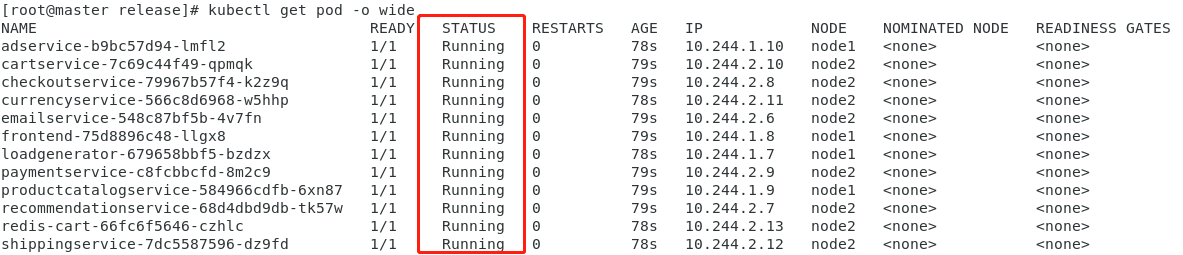
\includegraphics[width=1\textwidth]{figures/chapter2/nodes.png}
	\caption{Kubernetes资源pod列表}
	\label{fig:2-Kubernetes资源pod列表}
\end{figure}

\subsection{为微服务启用Istio支持}
进入了 `microservices-demo` 目录,并在 `istio-manifests` 目录中找到了 Istio 相关的 YAML 文件。通过使用 `kubectl apply` 命令,并指定 YAML 文件的路径,我们在集群中创建了 Istio 相关的资源,如 ServiceEntry、Gateway 和 VirtualService。使用以下命令创建了 Istio 资源:
\begin{lstlisting}[language=bash]
[root@master microservices-demo]# pwd
/root/online-boutique/microservices-demo

[root@master microservices-demo]# ls istio-manifests/
allow-egress-googleapis.yaml  frontend-gateway.yaml  frontend.yaml

[root@master microservices-demo]# kubectl apply -f ./istio-manifests
\end{lstlisting}
最后,我们获取了入口网关的 IP 地址并在浏览器中打开前端服务:
\begin{lstlisting}[language=bash]
[root@master microservices-demo]# INGRESS_HOST="$(kubectl -n istio-system get service istio-ingressgateway -o jsonpath='{.status.loadBalancer.ingress[0].ip}')"

[root@master microservices-demo]# echo "$INGRESS_HOST"

[root@master microservices-demo]# kubectl get service -n istio-system istio-ingressgateway -o wide
\end{lstlisting}

\subsection{访问首页与功能验证}
我们使用 `kubectl` 命令获取 Istio Ingress Gateway 的 IP 地址,并将其保存在 `INGRESS\_HOST` 变量中。然后,打印出该变量的值,以便在浏览器中使用。最后,使用 `kubectl get service` 命令获取 Istio Ingress Gateway 的详细信息,包括端口映射和所在节点等。在浏览器中打开 `INGRES\_HOST`,看到前端服务。在浏览器地址栏中输入 `http://<INGRESS\_HOST>/`,即可访问在线精品应用的前端界面。
删除 frontend-external 服务。frontend-external 服务是一个 LoadBalancer 服务,它暴露了前端。由于正在使用 Istio 的入口网关,不再需要这个 LoadBalancer 服务了。删除frontend-external服务,运行:
\begin{lstlisting}[language=bash]
[root@master ~]# kubectl get svc | grep frontend-external
frontend-external       LoadBalancer   10.102.0.207     192.168.110.191   80:30173/TCP   4d15h

[root@master ~]# kubectl delete svc frontend-external
service "frontend-external" deleted

[root@master ~]# kubectl get svc | grep frontend-external
\end{lstlisting}
Online Boutique 应用清单还包括一个负载发生器,它正在生成对所有服务的请求——这是为了让我们能够模拟网站的流量。
\begin{figure}[htb]
	\centering
	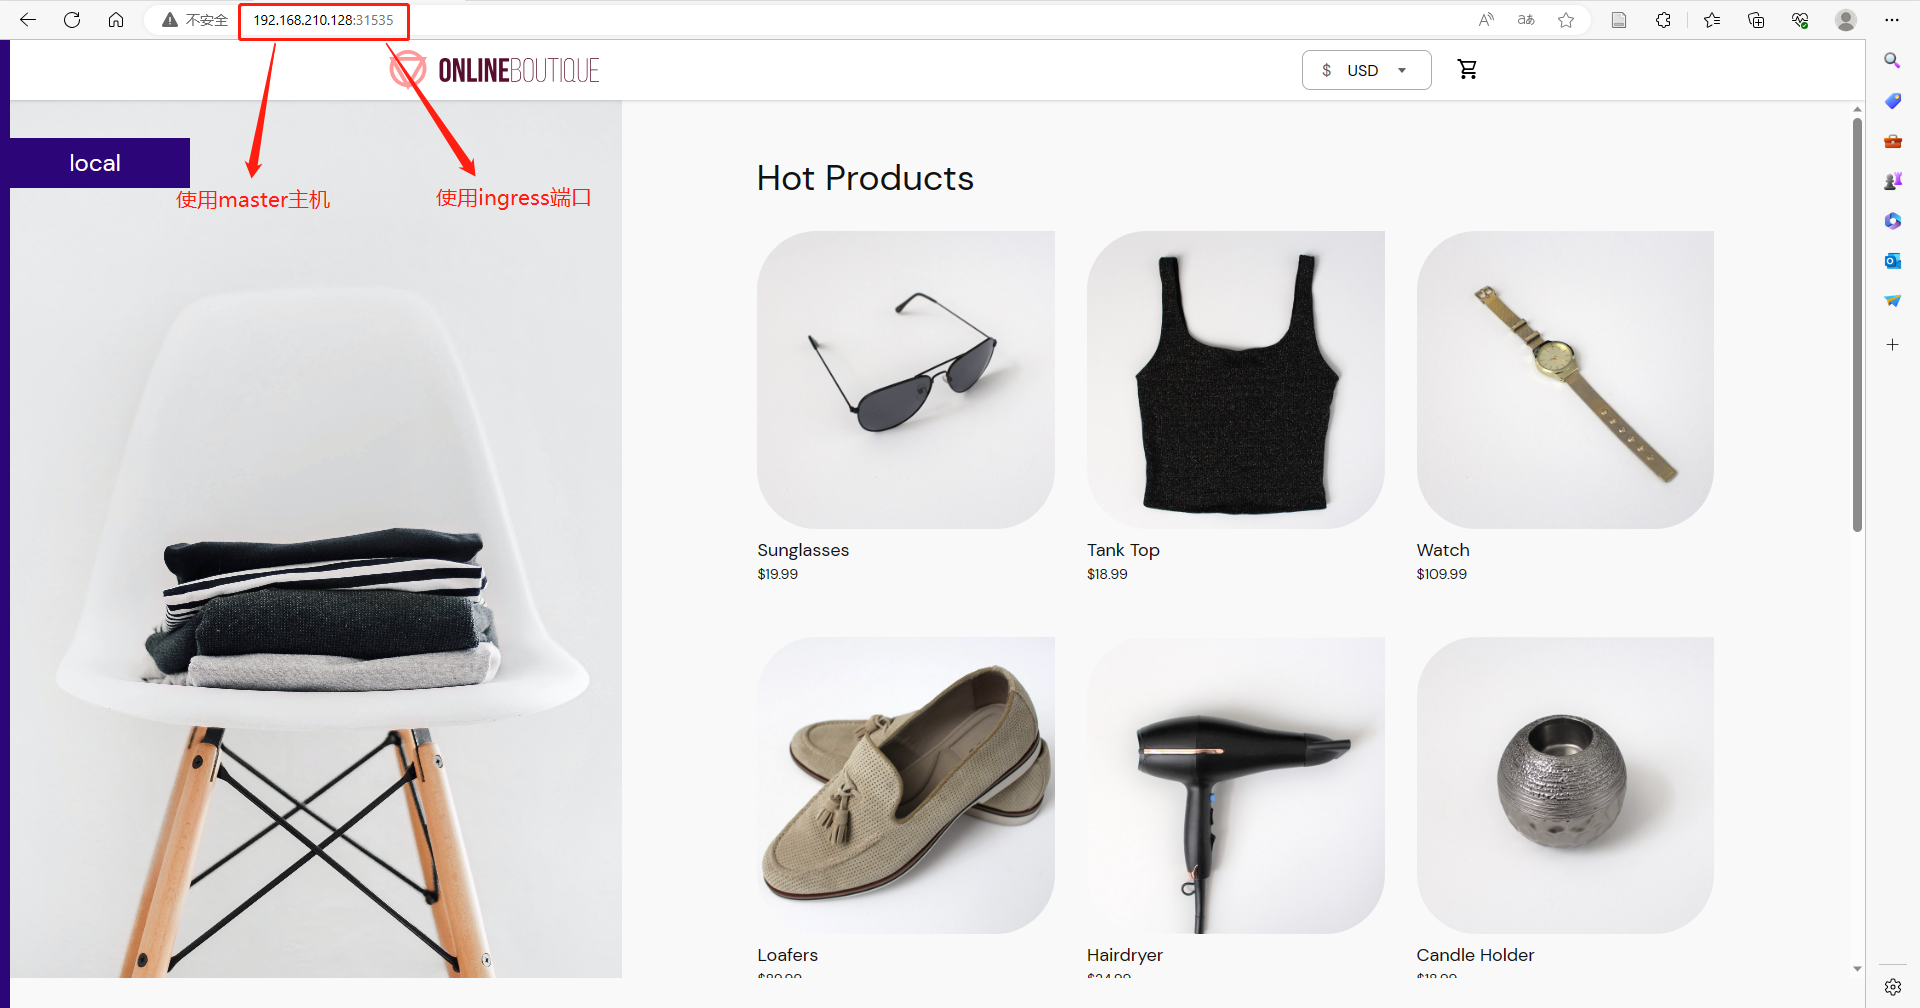
\includegraphics[width=1.0\textwidth]{figures/chapter2/Online Boutique.png}
	\caption{Online Boutique前端界面,使用ingress入口网关访问}
	\label{fig:2-Online Boutique前端界面}
\end{figure}
在Kubernetes Dashboard中查看online boutique命名空间下的服务,以adservice为例:
\begin{figure}[htb]
	\centering
	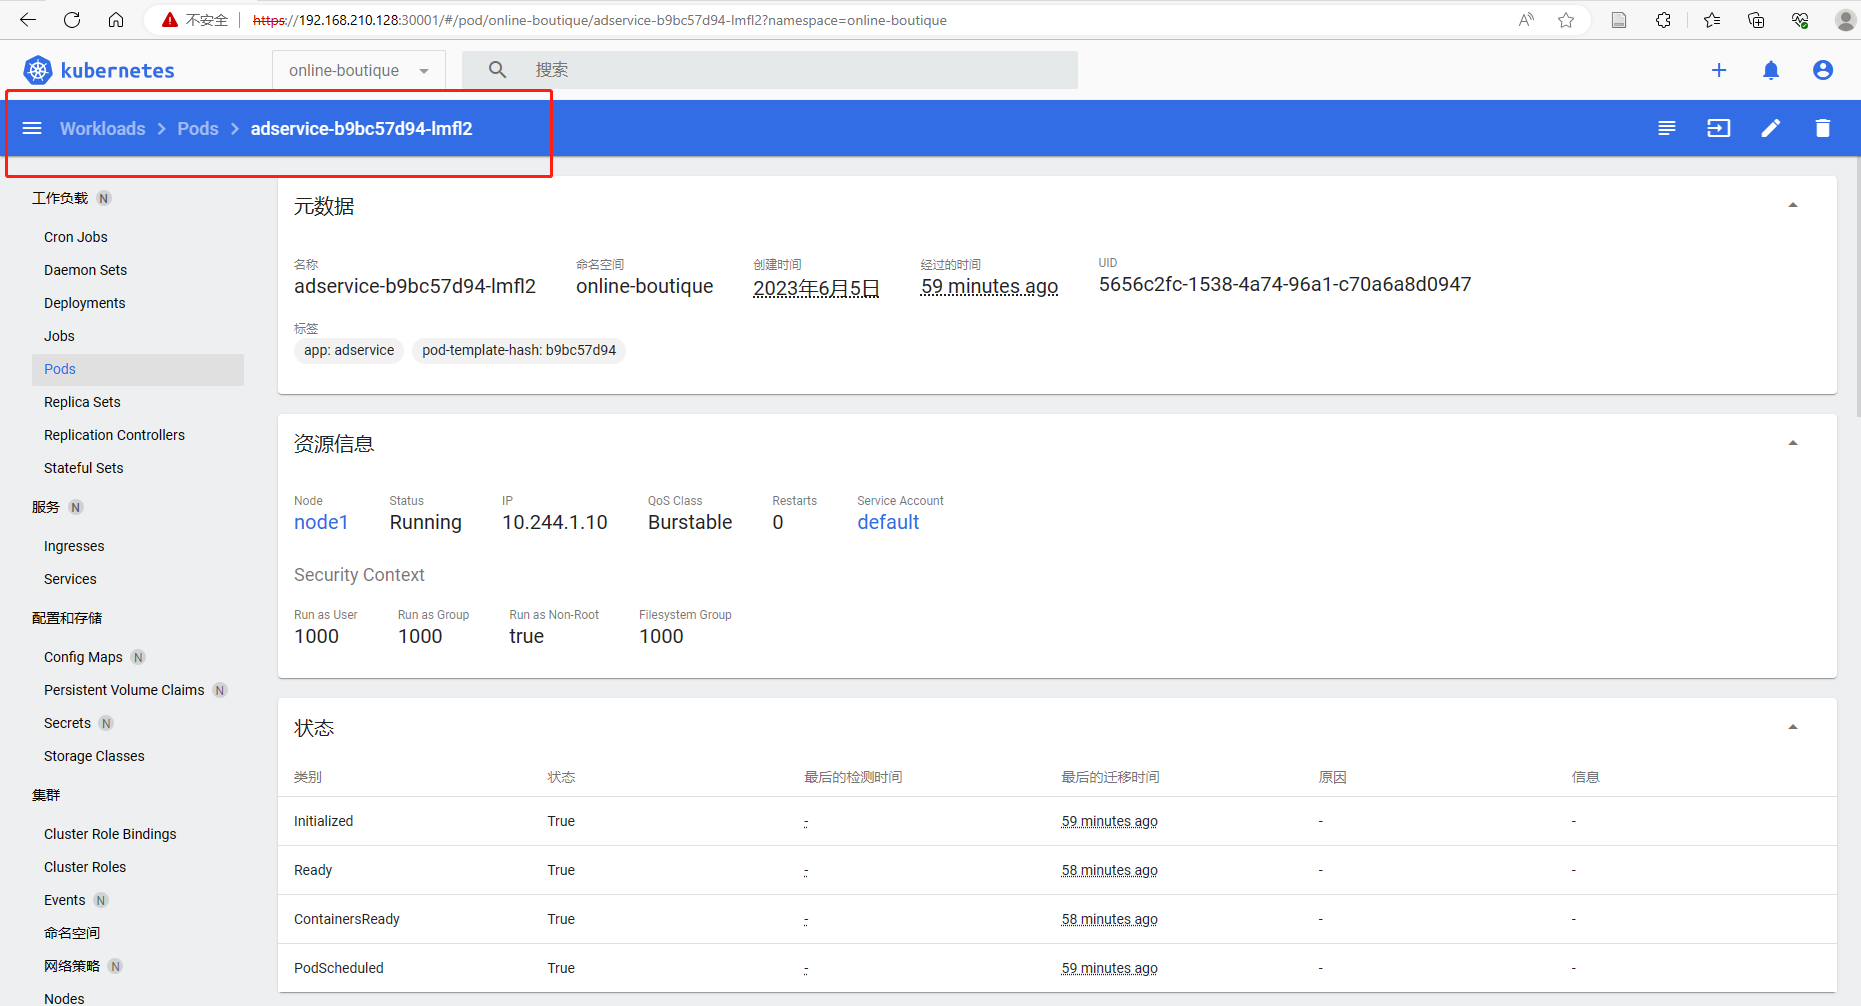
\includegraphics[width=1.0\textwidth]{figures/chapter2/online boutique on dashboard.png}
	\caption{online boutique命名空间下的服务,以adservice为例}
	\label{fig:2-online boutique命名空间下的服务,以adservice为例}
\end{figure}

\chapter{服务治理与监控}
\section{服务网络架构与传统网络架构对比与分析}
在现代微服务架构中,服务网络架构起着至关重要的作用。与传统的网络架构相比,服务网络架构引入了许多新的概念和技术,以更好地满足微服务应用的需求。本节将对服务网络架构与传统网络架构进行对比与分析,并探讨它们的优势和劣势。

\subsection{传统网络架构}

传统的网络架构通常基于三层模型,即应用层、传输层和网络层。在这种架构中,应用程序通过传输层协议(如 TCP 或 UDP)进行通信,并依赖于网络层协议(如 IP)进行数据传输。这种架构主要面向主机和网络之间的通信,而不太适用于微服务架构中的服务间通信。

在传统网络架构中,通信通常是基于主机和端口的,服务的位置和可用性对应用程序来说是透明的。这导致了以下一些问题:

\begin{itemize}
	\item \textbf{单点故障(SPOF):} 传统架构中的应用程序通常会直接连接到特定主机和端口。如果该主机或端口不可用,应用程序将无法正常工作,导致单点故障。
	\item \textbf{服务发现困难: }应用程序需要手动配置目标服务的主机和端口信息,这在大规模微服务系统中变得非常繁琐和复杂。随着服务数量的增加和动态变化,手动管理服务发现变得几乎不可行。
	\item \textbf{无法适应动态环境:} 传统架构很难适应动态环境中服务的频繁启动、停止和迁移。应用程序需要实时感知服务的变化,并相应地更新配置信息,这对于开发人员来说是一项巨大的挑战。
\end{itemize}

\subsection{服务网络架构}

服务网络架构通过引入服务代理和服务注册等概念,提供了一种更灵活、可扩展和可靠的服务间通信方式。在服务网络架构中,服务通过代理进行通信,代理负责处理服务发现、负载均衡、故障处理等任务。

以下是服务网络架构的一些关键概念和技术:

\begin{itemize}
	\item \textbf{服务代理: }服务代理是位于服务之间的中间层,它处理服务发现、负载均衡、熔断等功能。代理与每个服务建立连接,并代表应用程序进行通信,从而解耦了应用程序与具体服务之间的直接依赖关系。
	\item \textbf{服务注册: }服务注册是将服务实例的元数据(如主机和端口信息)注册到中心注册表中的过程。注册表充当服务发现的中心,应用程序可以查询注册表来获取目标服务的位置和可用性信息。
	\item \textbf{负载均衡: }服务代理可以根据负载均衡算法将请求分发到多个服务实例中,以实现负载均衡和高可用性。常见的负载均衡算法包括轮询、随机和加权轮询等。
	\item \textbf{熔断:} 熔断是一种故障处理机制,当目标服务发生故障或超过一定阈值时,服务代理会中断对该服务的请求,以避免故障的扩散和影响到其他服务。
\end{itemize}

服务网络架构相对于传统网络架构具有许多优势:

\begin{itemize}
	\item \textbf{高可用性和弹性:} 通过负载均衡和熔断等机制,服务网络架构能够提供高可用性和弹性,即使在某些服务实例故障的情况下,应用程序仍然可以正常工作。
	\item \textbf{动态服务发现:} 服务注册和服务发现机制使得应用程序能够动态地发现和连接到目标服务,无需手动配置主机和端口信息。这对于大规模微服务系统的管理和扩展非常重要。
	\item \textbf{灵活的部署和扩展: }服务网络架构使得服务的部署和扩展变得更加灵活和简化。服务可以独立部署和扩展,而无需修改应用程序的配置。
\end{itemize}

综上所述,服务网络架构相对于传统网络架构在微服务架构中具有许多优势,并且能够更好地满足微服务应用的需求。通过引入服务代理、服务注册和负载均衡等概念,服务网络架构实现了服务之间的解耦和动态发现,从而提高了系统的可靠性、可扩展性和可维护性。

本节主要实现一些监控(Prometheus)、追踪(Zipkin)、数据可视化工具(Grafana)和服务拓扑结构(Kiali)。
\section{熔断、限流、认证、授权的问题分析}
\subsection{熔断}
熔断是一种故障处理机制,用于保护系统免受服务故障的影响。当服务的错误率超过预定阈值时,熔断机制将临时中断对该服务的请求,以避免故障的扩散和对系统性能的负面影响。

监控熔断的关键是收集并分析与服务调用相关的指标。这些指标可以包括请求错误率、响应时间、失败率等。通过监控这些指标,可以及时检测到服务的故障情况,并触发熔断机制。

在解决熔断问题时,可以采取以下几个可行的解决思路:
\begin{itemize}
	\item \textbf{设置故障阈值}: 根据服务的性能和可靠性需求,设置适当的故障阈值。当服务的错误率超过该阈值时,触发熔断机制。
	\item \textbf{实施回退策略:} 当服务被熔断时,可以采取回退策略,例如返回默认值或从缓存中获取数据。这样可以确保在服务不可用时,仍能提供一定程度的功能。
	\item \textbf{自动恢复机制:} 一旦服务的错误率降低到可接受的水平,熔断机制应自动恢复服务,并逐渐增加请求量,以确保服务的可用性。
	\item \textbf{监控和报警系统}: 配置监控和报警系统来实时监测服务的错误率和熔断状态。当触发熔断时,及时通知开发团队并采取相应的措施。
\end{itemize}
\subsection{限流}
限流是一种保护系统免受过载的机制,用于限制对服务的并发请求量或吞吐量。通过限制请求的数量,可以防止服务过载和资源耗尽。

监控限流的关键是收集和分析与请求量和资源利用率相关的指标。这些指标可以包括并发请求数、吞吐量、平均响应时间等。通过监控这些指标,可以及时发现并处理潜在的请求过载问题。

在解决限流问题时,可以考虑以下几个解决思路:
\begin{itemize}
	\item \textbf{设置请求配额: }根据系统的容量和资源限制,设置每个服务的最大并发请求数或吞吐量。超过限制的请求将被拒绝或延迟处理。
	\item \textbf{实施排队机制: }当请求量超过系统处理能力时,可以将请求放入队列中,并按照一定的策略进行处理。这样可以有效控制请求的处理速率,避免资源耗尽。
	\item \textbf{动态调整限流策略: }根据系统负载和性能指标,动态调整限流策略。例如,在高负载时降低限流阈值,以避免系统过载;在低负载时适当提高限流阈值,以提高系统的利用率。
	\item \textbf{监控和报警系统: }配置监控和报警系统来实时监测请求量和限流状态。当触发限流时,及时通知开发团队并采取相应的措施。
\end{itemize}

\subsection{认证与授权}
认证与授权是保护系统安全和数据机密性的关键机制。认证用于验证用户身份,而授权用于确定用户对系统资源的访问权限。

监控认证与授权的关键是收集和分析与用户身份验证和资源访问相关的指标。这些指标可以包括登录失败次数、授权错误次数、授权访问成功率等。通过监控这些指标,可以及时发现安全漏洞和异常访问行为。

在解决认证与授权问题时,可以采取以下几个解决思路:
\begin{itemize}
	\item \textbf{多因素认证: }引入多因素认证机制,例如使用密码和验证码的组合,以提高身份验证的安全性。
	
	\item \textbf{使用安全令牌: }使用安全令牌(如 JWT)进行认证和授权,以避免在每次请求时都进行身份验证和授权。
	
	\item \textbf{实施权限管理: }管理用户的访问权限,并确保只有授权用户能够访问系统的特定资源。
	
	\item \textbf{监控和审计系统: }配置监控和审计系统来记录认证和授权的操作日志,并定期进行审查和分析,以发现异常访问行为。
\end{itemize}
\subsection{链路追踪}
链路追踪是一种分布式系统的监控技术,用于跟踪和分析请求在不同服务之间的流动和处理情况,以便识别和解决潜在的性能瓶颈和故障。

监控链路追踪的关键是收集和分析与请求流程、服务调用和响应时间相关的指标。这些指标可以包括请求的唯一标识符、请求的起始时间和结束时间、每个服务的处理时间等。通过监控这些指标,可以可视化请求的流程并分析服务间的调用关系。

在解决链路追踪问题时,可以考虑以下几个解决思路:
\begin{itemize}
	\item \textbf{使用分布式追踪系统: }集成分布式追踪系统(如 Jaeger、Zipkin)来收集和分析请求的链路信息。这些系统可以自动记录和跟踪请求在不同服务之间的流动情况。
	
	\item \textbf{添加唯一标识符:} 在每个请求中添加唯一标识符,并将其传递给后续的服务。这样可以跟踪请求在不同服务间的流动,并分析每个服务的处理时间。
	
	\item \textbf{可视化链路图: }根据收集的链路数据,生成可视化的链路图,显示请求在不同服务间的流动和处理情况。这样可以帮助开发团队快速定位性能瓶颈和故障点。
	
	\item \textbf{分析和优化: }基于链路追踪数据进行分析,找出潜在的性能瓶颈和故障点,并采取相应的优化措施,以提高系统的性能和可靠性。
\end{itemize}
\subsection{可观察性与指标}
由于采用了 sidecar 部署模式,即 Envoy 代理运行在应用实例旁边并拦截流量,这些代理也收集指标。

Envoy 代理收集的指标可以帮助我们获得系统状态的可见性。获得系统的这种可见性是至关重要的,因为我们需要了解正在发生的事情,并授权运维人员对应用程序进行故障排除、维护和优化。

Istio 生成三种类型的遥测数据,为网格中的服务提供可观察性\cite{istio-data}:
\begin{itemize}
	\item 指标度量(Metric)
	\item 分布式追踪
	\item 访问日志
\end{itemize}
Istio 基于四个黄金信号生成指标:延迟、流量、错误和饱和度。
\begin{itemize}
	\item 延迟表示服务一个请求所需的时间。这个指标应该分成成功请求(如 HTTP 200)和失败请求(如 HTTP 500)的延迟。
	\item 流量是衡量对系统的需求有多大,它是以系统的具体指标来衡量的。例如,每秒的 HTTP 请求,或并发会话,每秒的检索量,等等。
	\item 错误用来衡量请求失败的比率(例如 HTTP 500)。
	\item 饱和度衡量一个服务中最紧张的资源有多满。例如,线程池的利用率。
\end{itemize}
这些指标是在不同的层面上收集的,首先是最细的,即 Envoy 代理层面,然后是服务层面和控制平面的指标。本节接下来的部分针对服务拓扑发现与链路追踪、性能监控与可观测性两个层面配置和使用各种可观察性、分布式追踪、数据可视化工具。
\section{性能监控与可观测性}
在性能监控和可观测性分析中,Grafana和Prometheus是两个重要的工具,它们通常被一起使用来构建全面的监控和分析系统。

Prometheus是一个开源的监控系统和时间序列数据库,专门用于收集、存储和查询系统的指标数据。它支持灵活的数据模型和查询语言,能够高效地处理大量的时间序列数据。Prometheus采用了基于拉取的方式,周期性地从各个目标(如应用程序、服务、主机等)收集指标数据,并将其存储在本地的时间序列数据库中。它还提供了丰富的查询语言和表达式,用于实时监控和分析指标数据,例如计算平均值、聚合数据、设置报警规则等。

Grafana则是一个强大的数据可视化平台,用于展示和分析来自不同数据源的监控指标数据。Grafana支持多种数据源,其中包括Prometheus。它提供了直观的用户界面,用户可以根据需要创建自定义的仪表盘和面板,将不同数据源的指标数据可视化呈现出来。通过Grafana,用户可以轻松地创建图表、图形、表格等各种可视化元素,以实时、直观的方式展示系统的性能指标和趋势。此外,Grafana还支持设置报警规则和通知机制,以便在系统达到预设的阈值时发送警报通知。

综合使用Prometheus和Grafana,可以建立一个完整的性能监控和可观测性分析系统。Prometheus负责数据的收集、存储和查询,而Grafana则负责将这些数据进行可视化展示和分析。用户可以通过Grafana创建个性化的仪表盘,实时监控系统的各项指标,并根据需要进行深入的数据分析和性能优化。这样的组合能够帮助用户更好地了解系统的运行状态、发现潜在的问题,并及时采取相应的措施来提高系统的性能和稳定性。
\subsection{Prometheus 的配置与使用}
Prometheus 是一个开源的监控系统和时间序列数据库,最初由 SoundCloud 开发并于2012年发布。它专为高度动态的分布式环境而设计,可以帮助用户监控系统和服务的性能指标、告警状态以及记录事件数据。

Prometheus 通过收集和存储时间序列数据来实现监控功能。它支持多种数据模型和查询语言,可以有效地存储大规模的时间序列数据,并提供强大的查询和聚合功能。Prometheus 使用拉取模型,周期性地从目标系统中获取指标数据,同时也支持推送模型,允许目标系统将数据主动推送给 Prometheus。

Prometheus 提供了灵活的告警规则配置,可以基于采集的指标数据定义自定义的告警条件,并在触发告警时发送通知。它还具有强大的可视化能力,通过内置的图形界面和集成的 Grafana 工具,用户可以实时监控和分析指标数据,创建仪表板和报表来展示系统的状态和趋势。

在 Istio 中,Prometheus 被用于记录指标,跟踪 Istio 和服务网格中应用程序的健康状况。它可以与 Istio 的各个组件集成,帮助用户实现对服务的监控、度量和告警。

要安装 Prometheus,我们可以使用 Istio 安装包中 /samples/addons 文件夹中的示例安装。
\begin{lstlisting}[language=bash][language=bash, caption={安装 Prometheus}]
[root@k8scloude1 ~]# cd istio-1.14.3/
[root@k8scloude1 istio-1.14.3]# cd samples/addons/
[root@k8scloude1 addons]# vim prometheus.yaml
\end{lstlisting}
可以看到安装 Prometheus 需要用到两个镜像:jimmidyson/configmap-reload:v0.5.0 和 prom/prometheus:v2.31.1
\begin{lstlisting}[language=bash][language=bash]
# 提前在 Kubernetes 的 worker 节点拉取所需镜像,以 k8scloude2 节点为例
[root@k8scloude2 ~]# docker pull jimmidyson/configmap-reload:v0.5.0
[root@k8scloude2 ~]# docker pull prom/prometheus:v2.31.1
\end{lstlisting}
安装 Prometheus:
\begin{lstlisting}[language=bash][language=bash]
[root@k8scloude1 addons]# kubectl apply -f prometheus.yaml
serviceaccount/prometheus created
configmap/prometheus created
clusterrole.rbac.authorization.k8s.io/prometheus created
clusterrolebinding.rbac.authorization.k8s.io/prometheus created
service/prometheus created
deployment.apps/prometheus created
\end{lstlisting}
检查 Prometheus 是否成功部署
\begin{lstlisting}[language=bash][language=bash]	
[root@k8scloude1 addons]# kubectl get deploy -n istio-system
NAME                   READY   UP-TO-DATE   AVAILABLE   AGE
istio-egressgateway    1/1     1            1           62m
istio-ingressgateway   1/1     1            1           62m
istiod                 1/1     1            1           62m
prometheus             1/1     1            1           12s
\end{lstlisting}
检查 Prometheus 运行状态
\begin{lstlisting}[language=bash][language=bash]	
[root@k8scloude1 ~]# kubectl get pod -n istio-system -o wide
NAME                                    READY   STATUS    RESTARTS   AGE   IP            NODE    NOMINATED NODE   READINESS GATES
istio-egressgateway-5f864bf78f-n4bs4    1/1     Running   0          62m   10.244.2.14   node2   <none>           <none>
istio-ingressgateway-78c7bbfc7c-wbtdd   1/1     Running   0          62m   10.244.2.15   node2   <none>           <none>
istiod-fcb96b864-87gcx                  1/1     Running   0          62m   10.244.1.11   node1   <none>           <none>
prometheus-6956c8c6c5-6zc94             2/2     Running   0          48s   10.244.1.12   node1   <none>           <none>
b-kz5sd                 1/1     Running   10         8d    10.244.112.137   k8scloude2
\end{lstlisting}
查看 Istio 系统中的 Prometheus 服务类型为 ClusterIP,无法从外部环境访问,修改 Prometheus 这个 service 的类型为 NodePort,这样外部环境就可以访问 Prometheus 。将 "type: ClusterIP" 修改为 "type: NodePort"
\begin{lstlisting}[language=bash][language=bash]
	kubectl edit service prometheus -n istio-system
\end{lstlisting}
\begin{lstlisting}[language=bash]
spec:
clusterIP: 10.102.117.137
clusterIPs:
- 10.102.117.137
internalTrafficPolicy: Cluster
ipFamilies:
- IPv4
ipFamilyPolicy: SingleStack
ports:
- name: http
port: 9090
protocol: TCP
targetPort: 9090
selector:
app: prometheus
component: server
release: prometheus
sessionAffinity: None
type: NodePort
status:
loadBalancer: {}
\end{lstlisting}
现在 Prometheus 这个 service 的类型为 NodePort,浏览器输入物理机 IP:pod端口号 即可访问 Prometheus 网页了
因为k8scloude1地址为192.168.210.168,所以我们可以在浏览器中打开 http://192.168.210.168:30225/,进入 Prometheus 仪表盘,输入istio\_requests\_total之后,点击Execute执行,就可以看到收集到的数据,如下图所示:

\begin{figure}[htb]
	\centering
	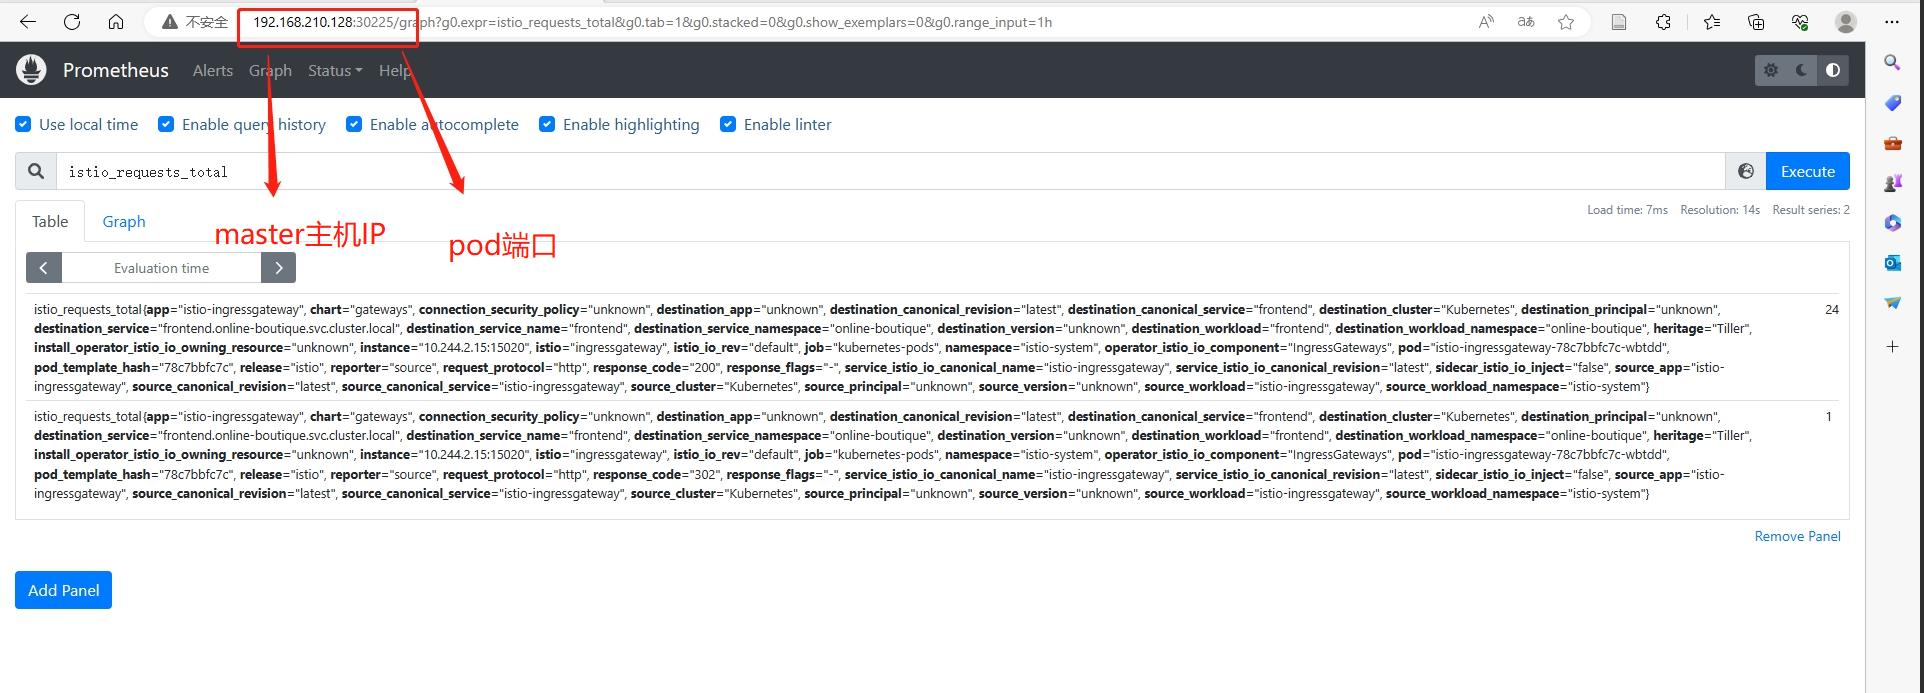
\includegraphics[width=1.0\textwidth]{figures/chapter2/prometheus.png}
	\caption{Prometheus监控仪表盘与使用}
	\label{fig:3-Prometheus监控仪表盘与使用}
\end{figure}
下面是一个来自 Prometheus 用户界面的示例元素:
\begin{lstlisting}[language=bash]
istio_requests_total{app="istio-ingressgateway", chart="gateways", connection_security_policy="unknown", destination_app="unknown", destination_canonical_revision="latest", destination_canonical_service="frontend", destination_cluster="Kubernetes", destination_principal="unknown", destination_service="frontend.online-boutique.svc.cluster.local", destination_service_name="frontend", destination_service_namespace="online-boutique", destination_version="unknown", destination_workload="frontend", destination_workload_namespace="online-boutique", heritage="Tiller", install_operator_istio_io_owning_resource="unknown", instance="10.244.2.15:15020", istio="ingressgateway", istio_io_rev="default", job="kubernetes-pods", namespace="istio-system", operator_istio_io_component="IngressGateways", pod="istio-ingressgateway-78c7bbfc7c-wbtdd", pod_template_hash="78c7bbfc7c", release="istio", reporter="source", request_protocol="http", response_code="200", response_flags="-", service_istio_io_canonical_name="istio-ingressgateway", service_istio_io_canonical_revision="latest", sidecar_istio_io_inject="false", source_app="istio-ingressgateway", source_canonical_revision="latest", source_canonical_service="istio-ingressgateway", source_cluster="Kubernetes", source_principal="unknown", source_version="unknown", source_workload="istio-ingressgateway", source_workload_namespace="istio-system"}
\end{lstlisting}
\subsection{Grafana 的配置与使用}
Grafana是一个开源的数据可视化和监控平台。它提供了丰富的数据查询、可视化和报警功能,可用于实时监控和分析各种数据源,包括时间序列数据、日志数据和数据库数据等。Grafana支持多种数据源,如Prometheus、InfluxDB、Elasticsearch等,可以根据需求创建自定义的仪表盘和面板,以便直观地展示数据指标和趋势。Grafana广泛应用于DevOps、系统监控、应用性能分析和可视化等领域,帮助用户实时监控系统状态、分析性能问题,并支持决策和故障排除。

运行以下命令来部署 Grafana 和预配置的仪表盘:
\begin{lstlisting}[language=bash][language=bash]
kubectl apply -f grafana.yaml
% 查看 Istio 系统中的 Pod
kubectl get pod -n istio-system
% 查看 Grafana 这个 service 的类型为 ClusterIP,无法从外部环境访问
kubectl get service -n istio-system
% 修改 Grafana 这个 service 的类型为 NodePort,这样外部环境就可以访问 Grafana
% 将 "type: ClusterIP" 修改为 "type: NodePort"
kubectl edit service grafana -n istio-system
% 现在 Grafana 这个 service 的类型为 NodePort,浏览器输入物理机 IP:31092 即可访问 Grafana 网页
kubectl get service -n istio-system
\end{lstlisting}

k8scloude1 机器的地址为 192.168.210.128,我们可以在浏览器中打开 \url{http://192.168.210.128:30729},进入 Grafana,点击搜索框和 istio 文件夹,查看已安装的仪表盘,如下图所示:
\begin{figure}[H]
	\centering
	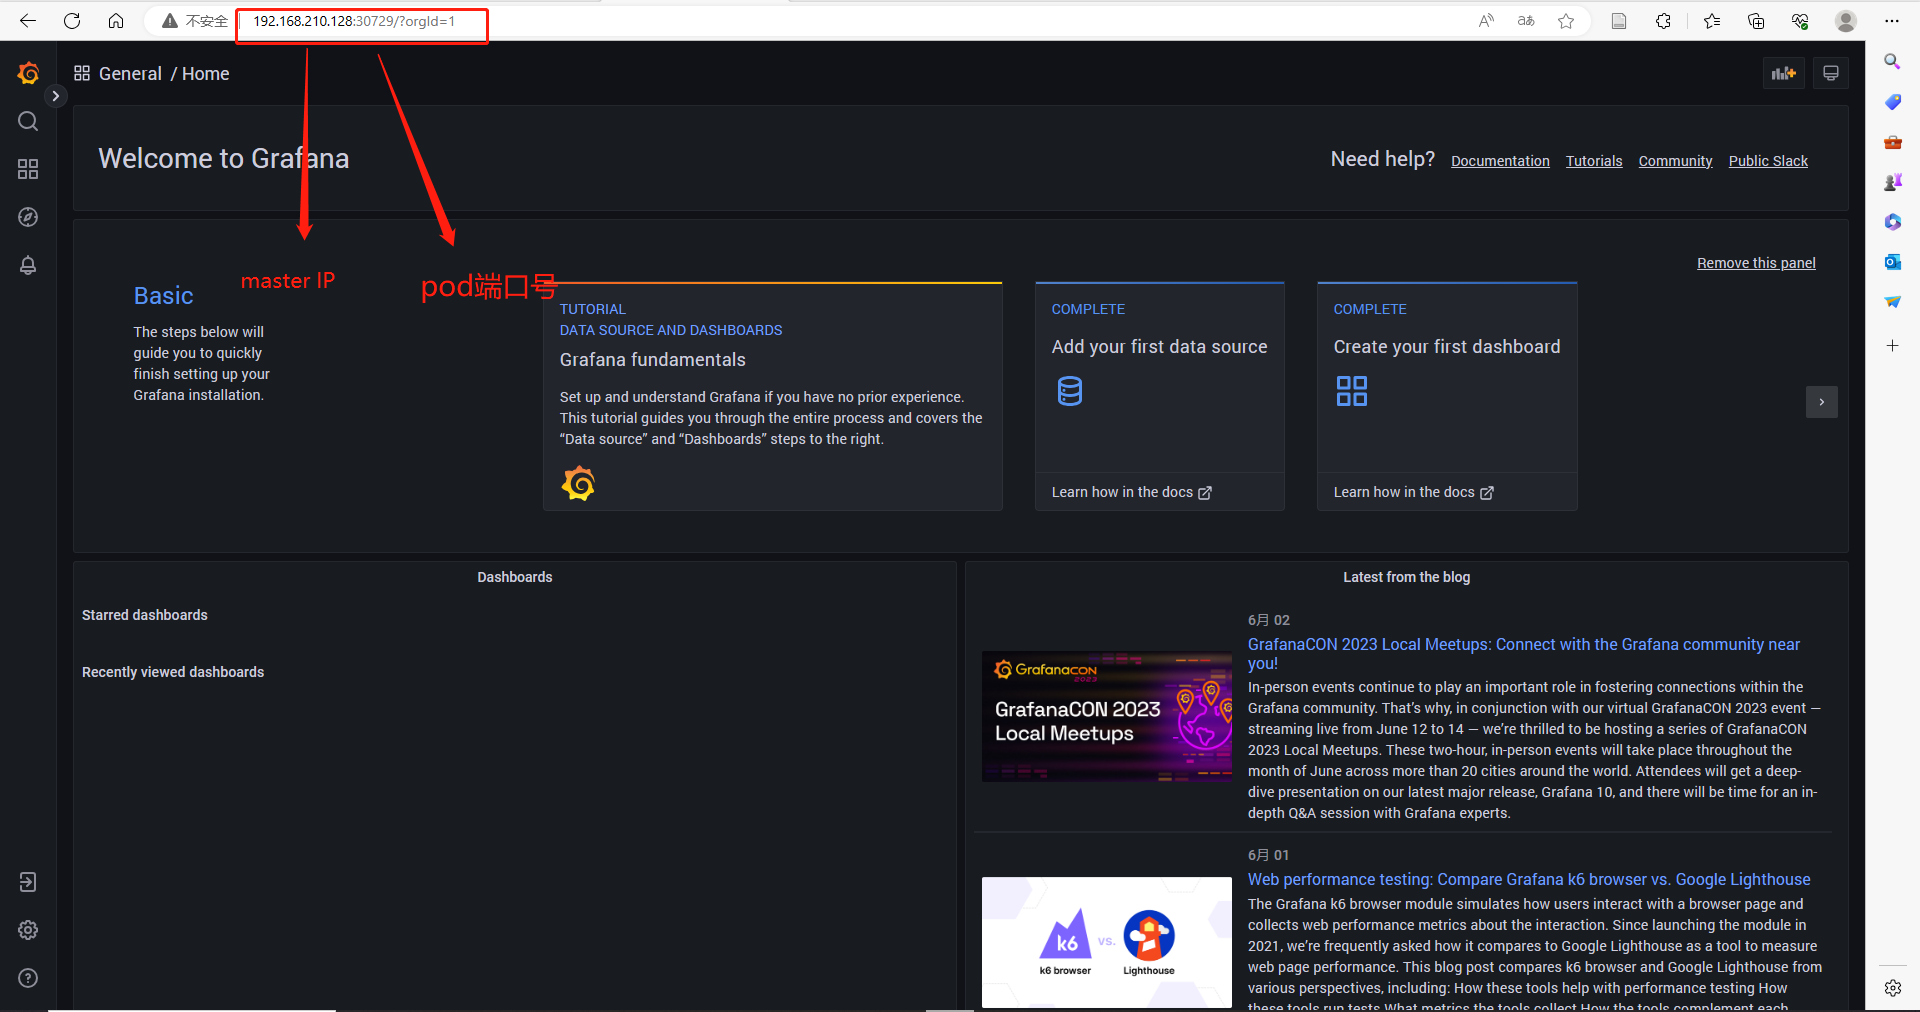
\includegraphics[width=1.0\textwidth]{figures/chapter2/grafana.png}
	\caption{Grafana监控仪表盘与使用}
	\label{fig:3-Grafana监控仪表盘与使用}
\end{figure}
Istio Grafana 安装时预配置了以下仪表盘:

Istio 控制平面仪表盘(Istio Control Plane Dashboard)可以监控 Istio 控制平面的健康和性能,展示控制平面的资源使用情况(内存、CPU、磁盘、Go routines),以及关于 Pilot、Envoy 和 Webhook 的信息。
\begin{figure}[H]
	\centering
	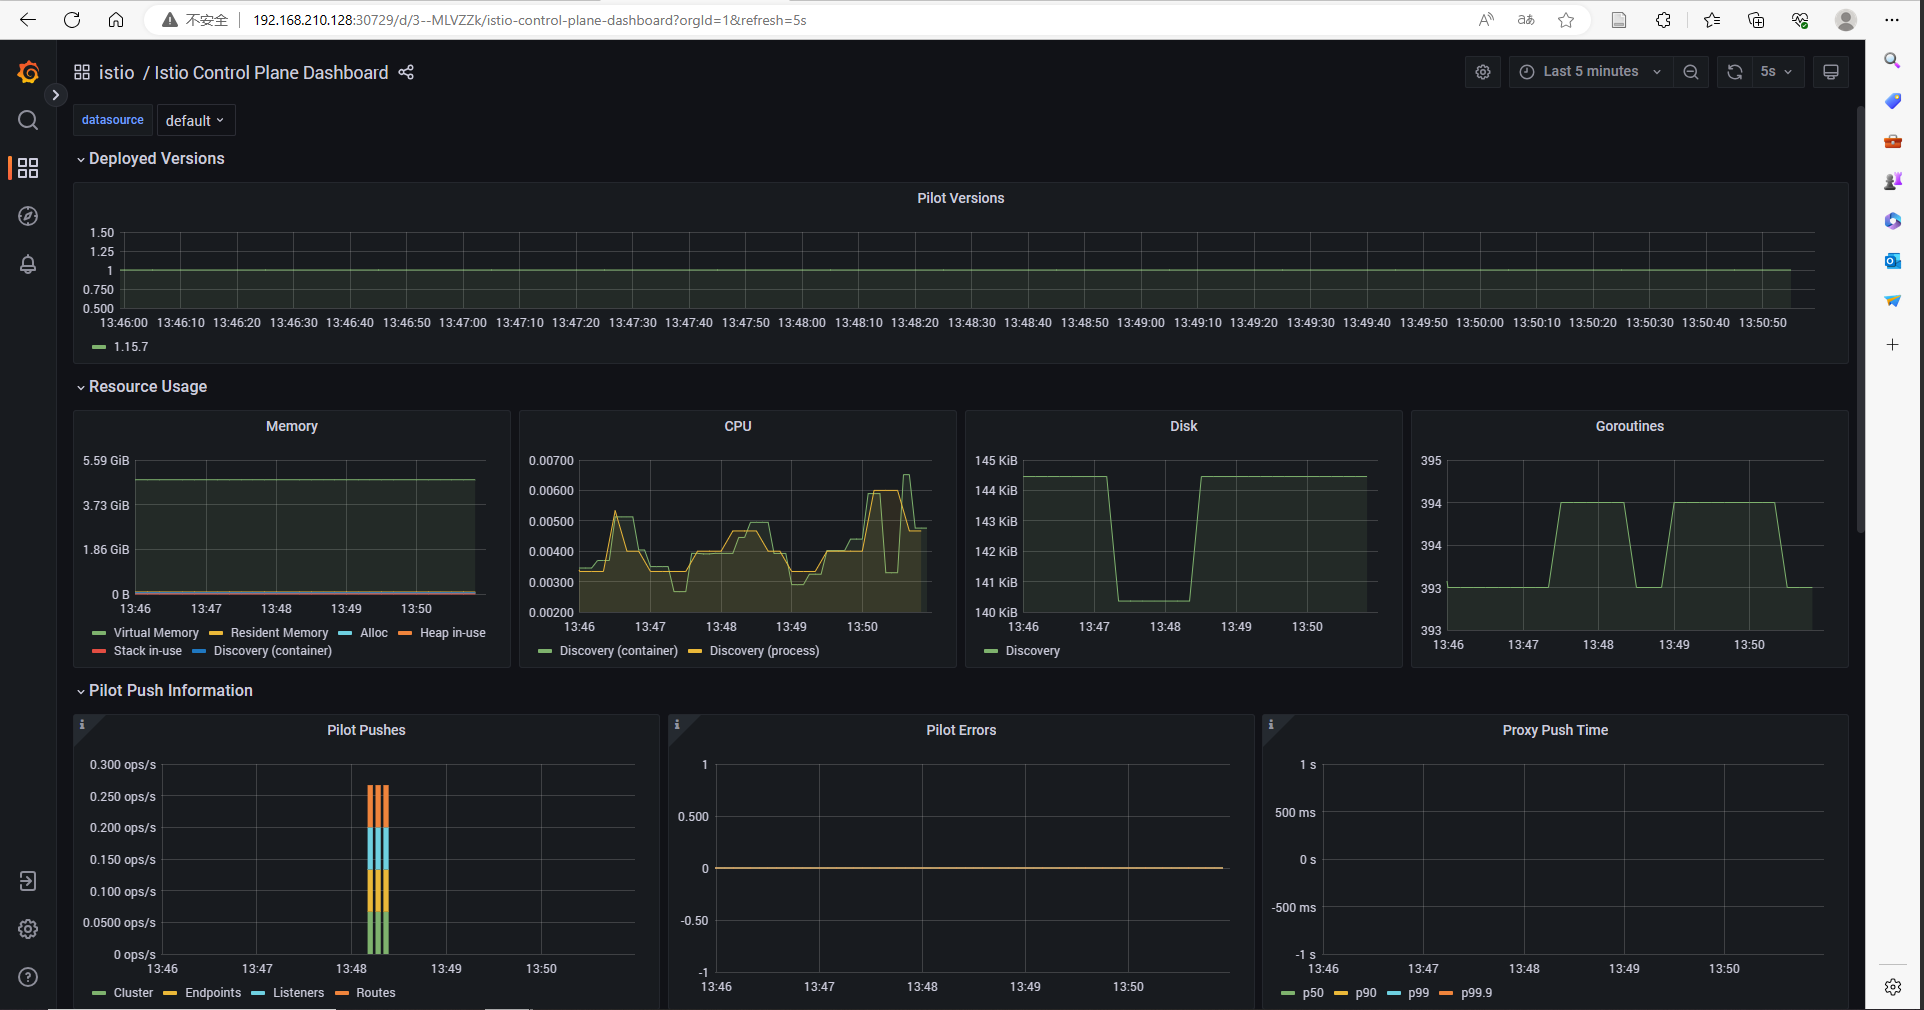
\includegraphics[width=1.0\textwidth]{figures/chapter2/CPA.png}
	\caption{Istio 控制平面仪表盘(Istio Control Plane Dashboard)}
	\label{fig:3-Istio 控制平面仪表盘(Istio Control Plane Dashboard)}
\end{figure}
Istio 网格仪表盘(Istio Mesh Dashboard)提供了在网格中运行的所有服务的概览。仪表盘包括全局请求量、成功率以及 4xx 和 5xx 响应的数量。
\begin{figure}[H]
	\centering
	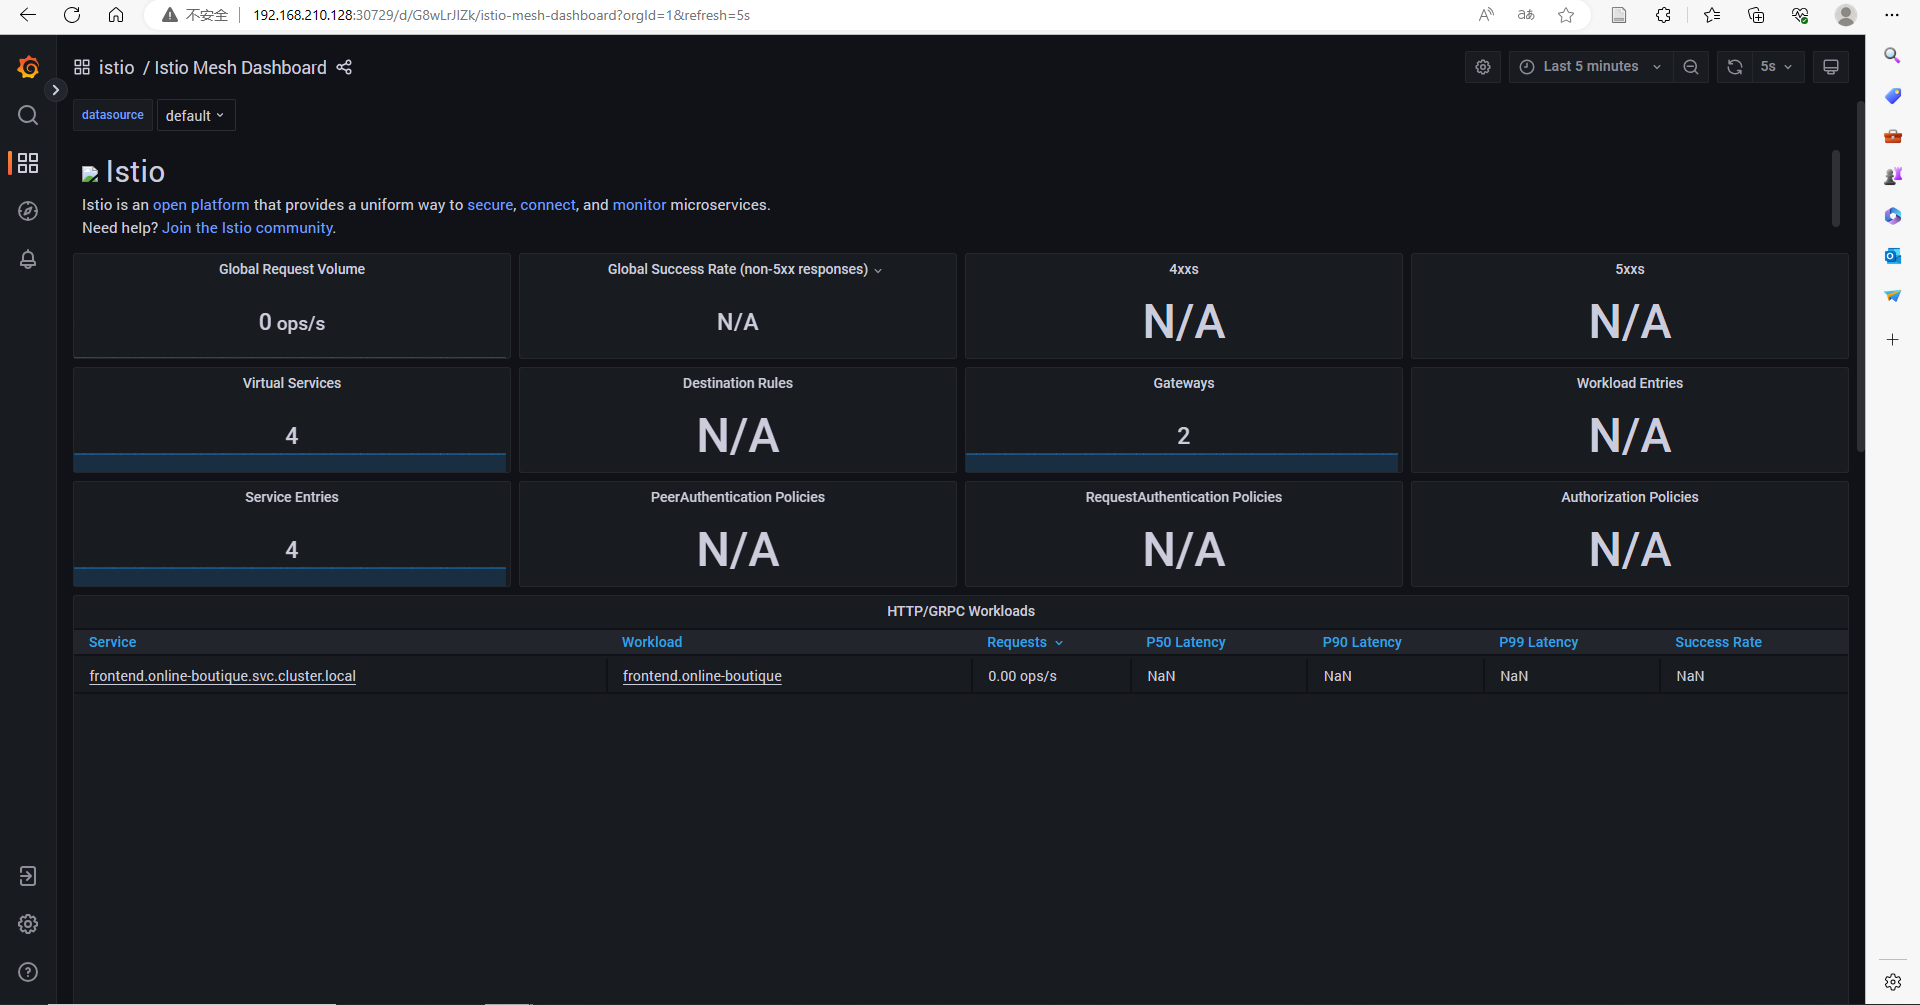
\includegraphics[width=1.0\textwidth]{figures/chapter2/MD.png}
	\caption{Istio 网格仪表盘(Istio Mesh Dashboard)}
	\label{fig:3-Istio 网格仪表盘(Istio Mesh Dashboard)}
\end{figure}
Istio 性能仪表盘(Istio Performance Dashboard)展示了 Istio 主要组件在稳定负载下的资源利用率。
\begin{figure}[H]
	\centering
	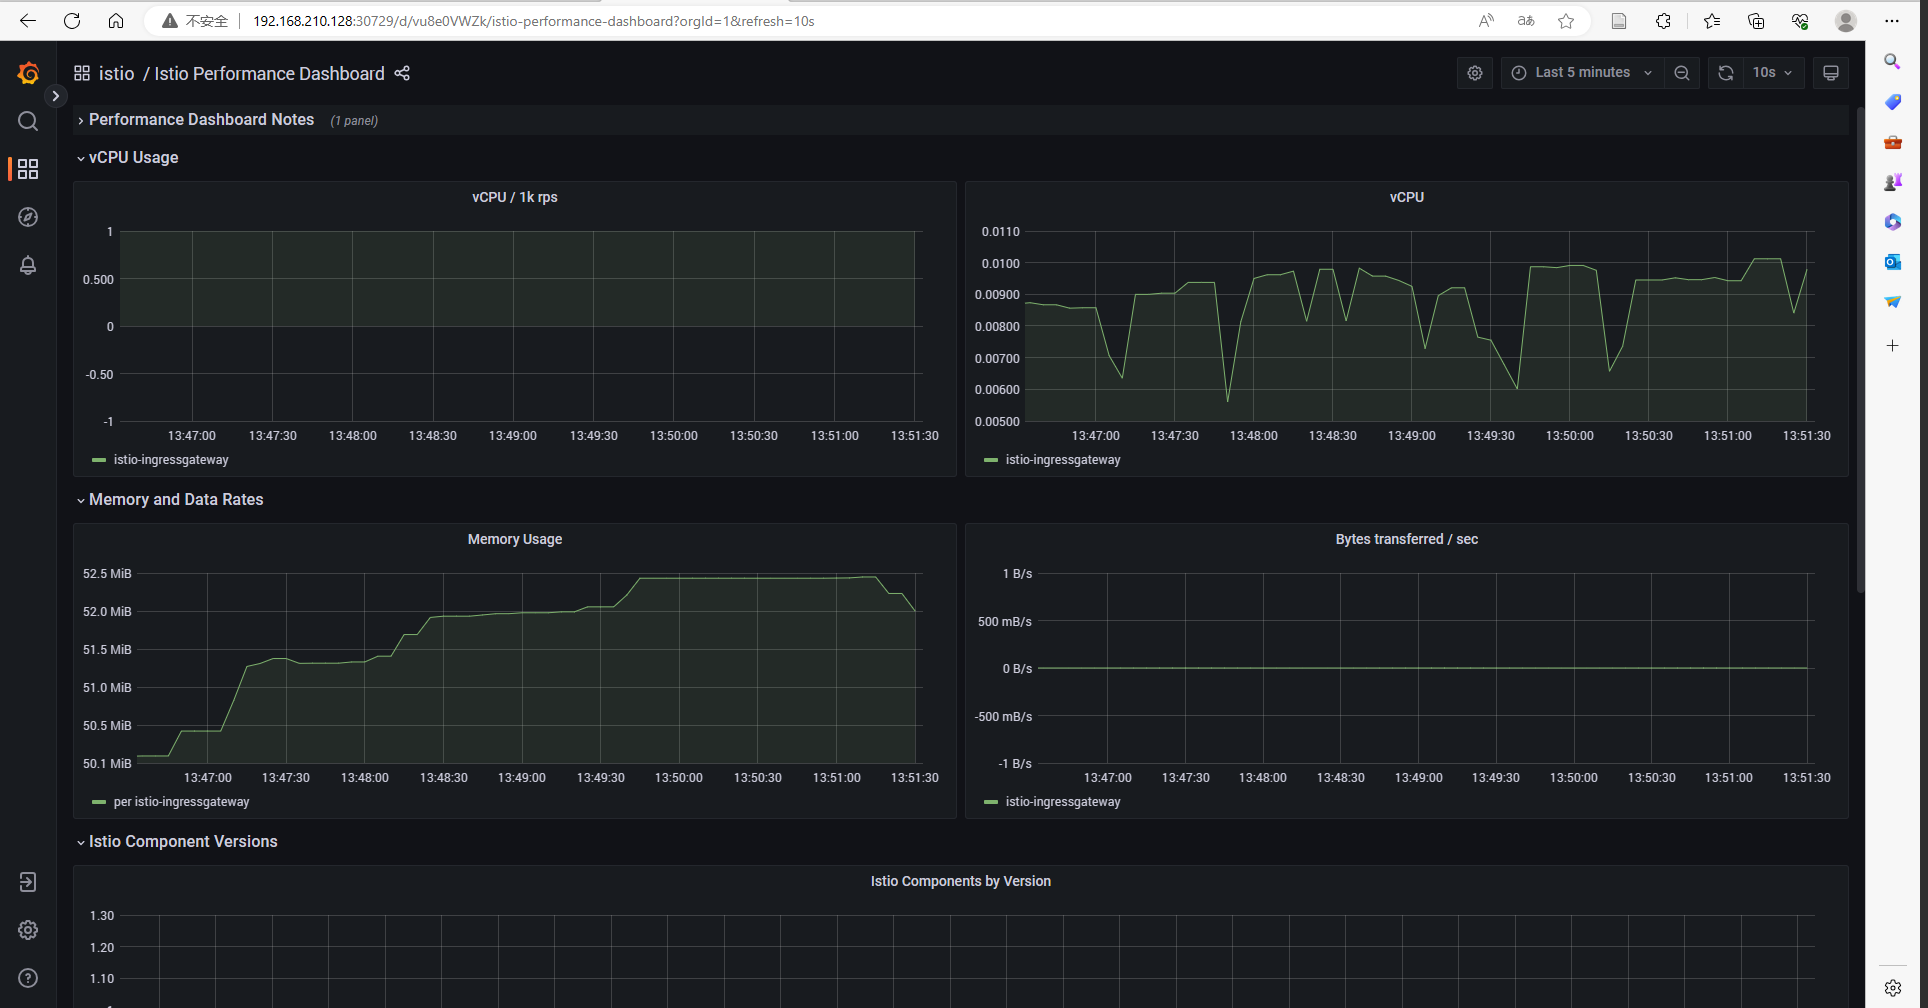
\includegraphics[width=1.0\textwidth]{figures/chapter2/PD.png}
	\caption{Istio 性能仪表盘(Istio Performance Dashboard)}
	\label{fig:3-Istio 性能仪表盘(Istio Performance Dashboard)}
\end{figure}
Istio 服务仪表盘(Istio Service Dashboard)允许查看服务的细节,可以获得关于请求量、成功率、持续时间的信息,以及显示按来源和响应代码、持续时间和大小的传入请求的详细图表。
\begin{figure}[H]
	\centering
	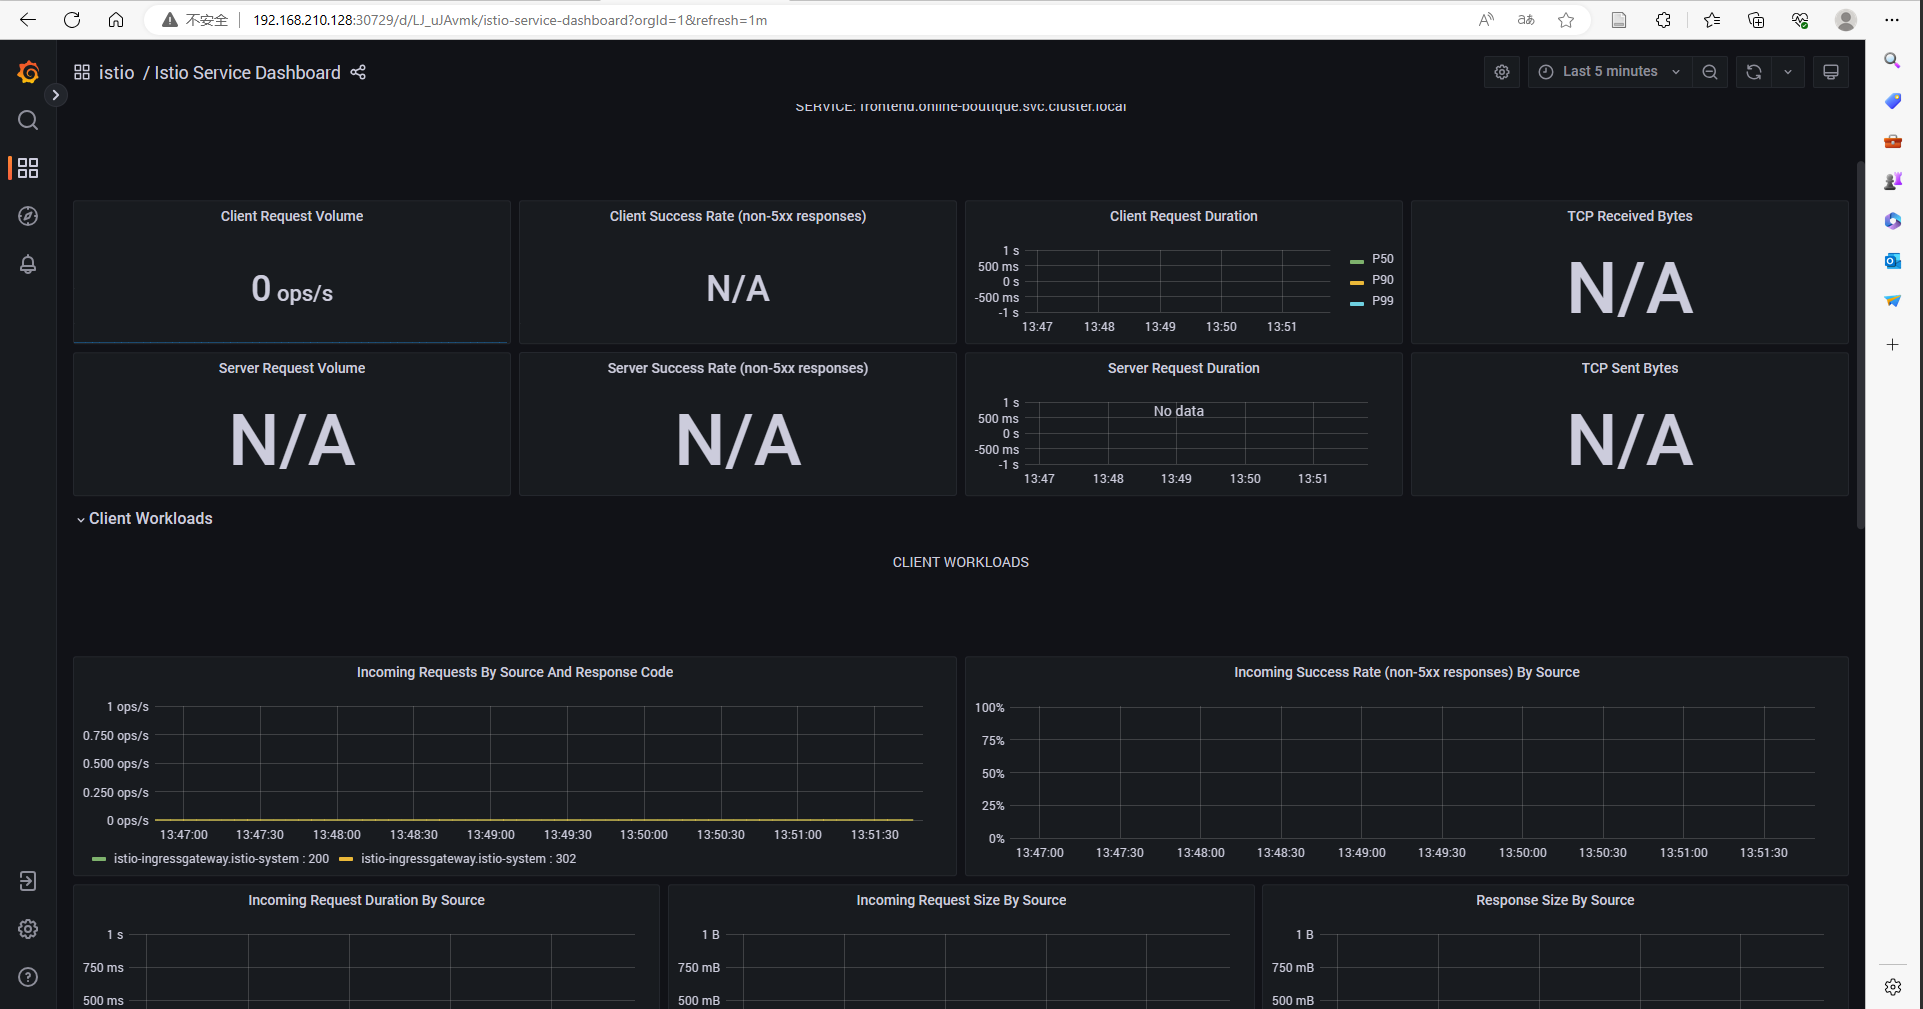
\includegraphics[width=1.0\textwidth]{figures/chapter2/SD.png}
	\caption{Istio 服务仪表盘(Istio Service Dashboard)}
	\label{fig:3-Istio 服务仪表盘(Istio Service Dashboard)}
\end{figure}
Istio Wasm 扩展仪表盘(Istio Wasm Extension Dashboard)显示与 WebAssembly 模块有关的指标,可以监控活动的和创建的 Wasm 虚拟机,关于获取删除 Wasm 模块和代理资源使用的数据。
\begin{figure}[H]
	\centering
	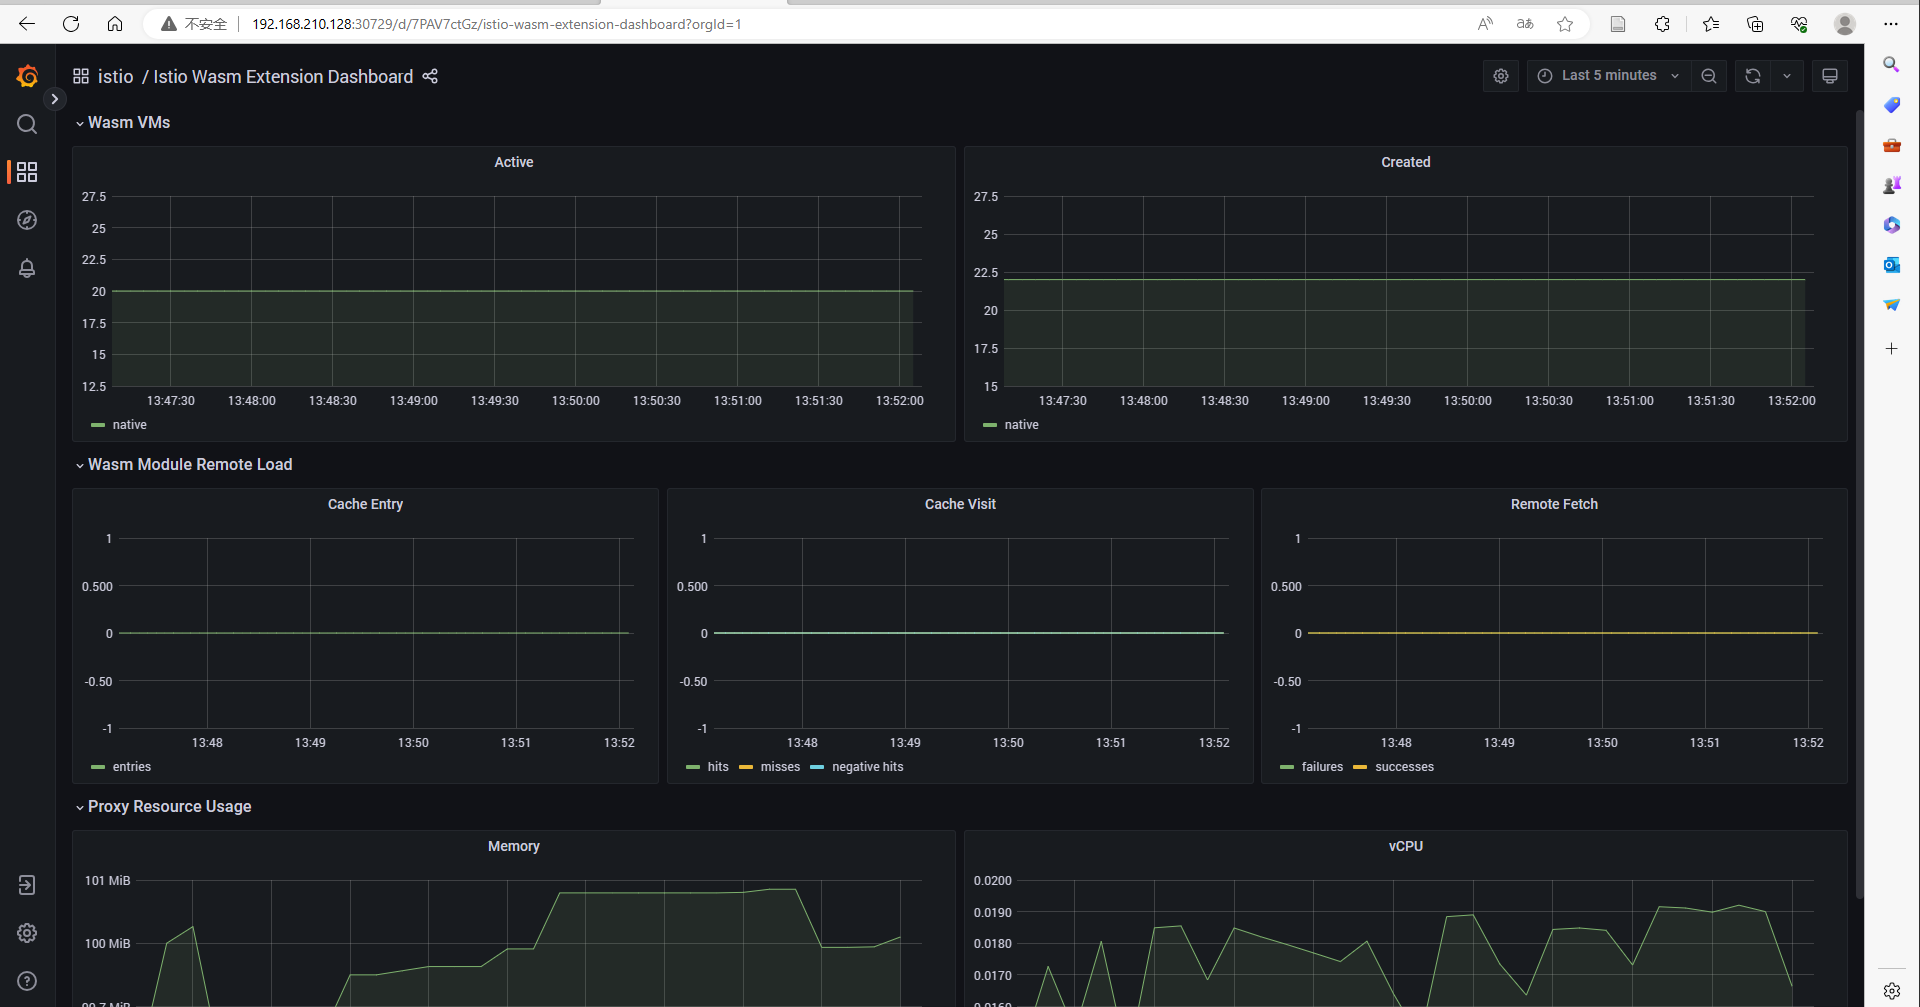
\includegraphics[width=1.0\textwidth]{figures/chapter2/WED.png}
	\caption{Istio Wasm 扩展仪表盘(Istio Wasm Extension Dashboard)}
	\label{fig:3-Istio Wasm 扩展仪表盘(Istio Wasm Extension Dashboard)}
\end{figure}
Istio 工作负载仪表盘(Istio Workload Dashboard)提供了一个工作负载的详细指标分类。
\begin{figure}[H]
	\centering
	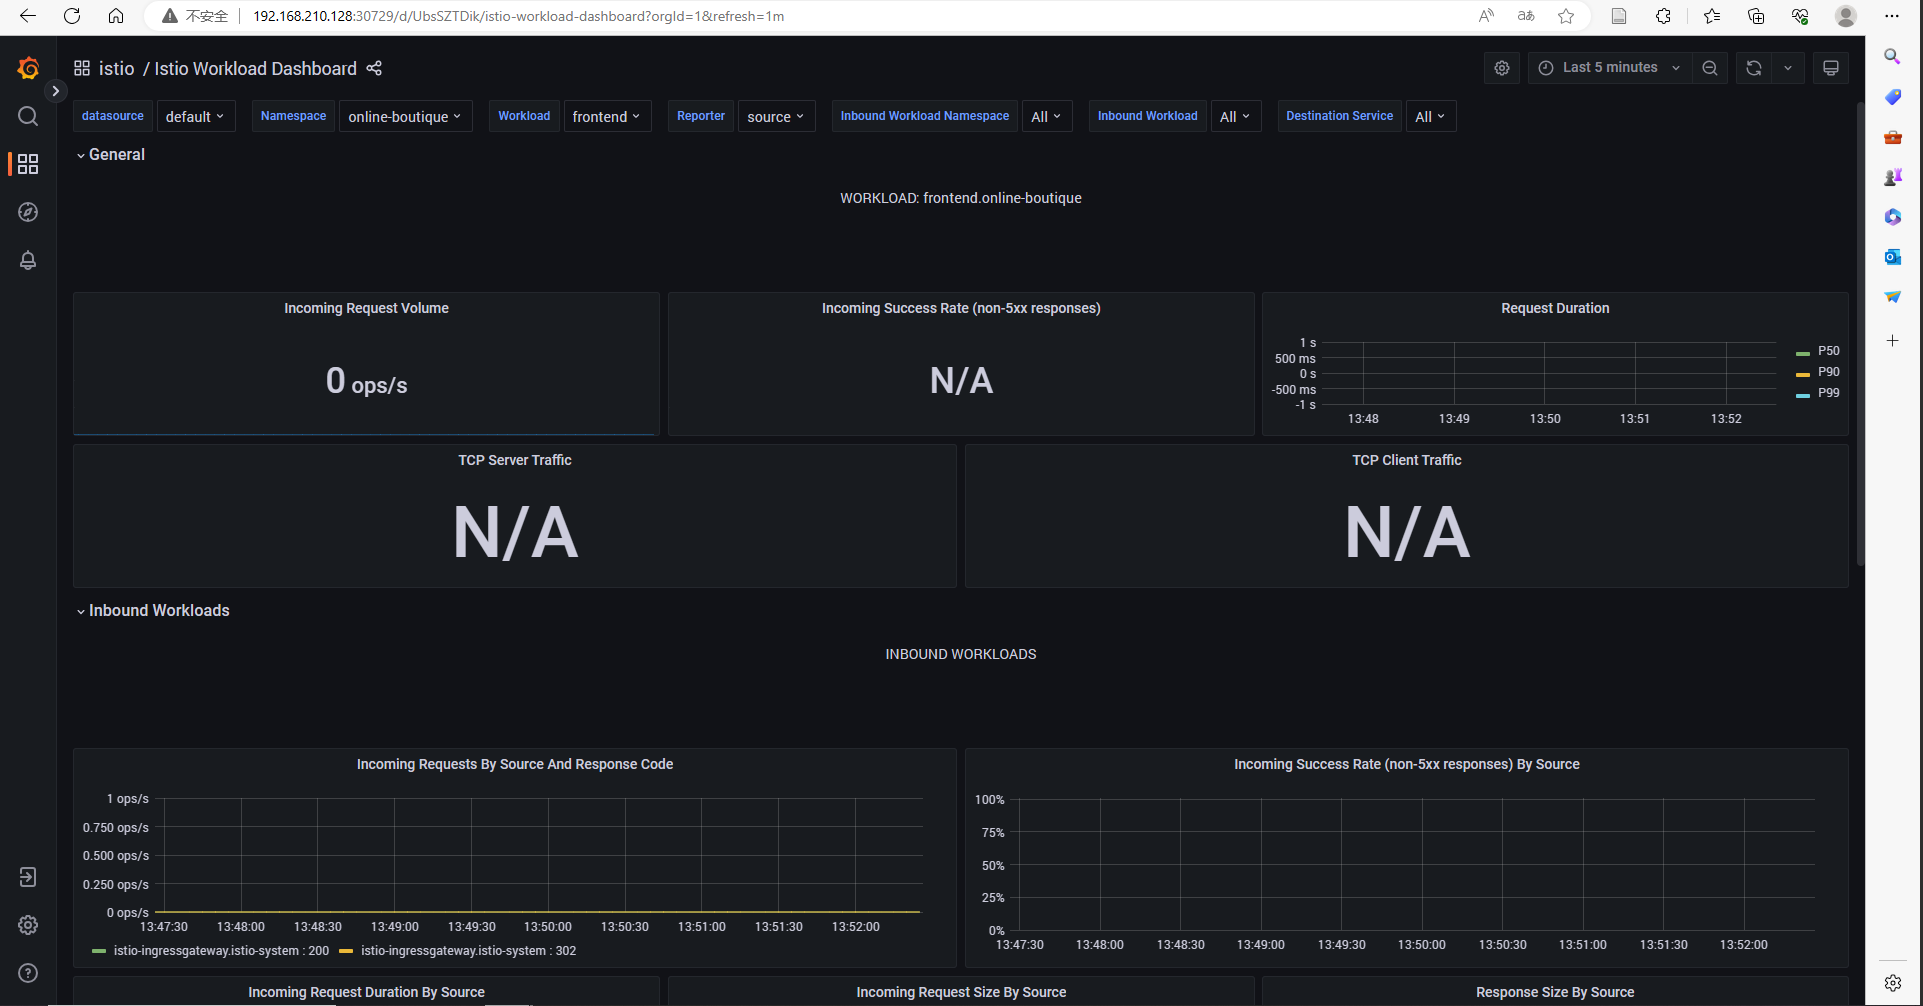
\includegraphics[width=1.0\textwidth]{figures/chapter2/WD.png}
	\caption{Istio 工作负载仪表盘(Istio Workload Dashboard)}
	\label{fig:3-Istio 工作负载仪表盘(Istio Workload Dashboard)}
\end{figure}
\section{服务拓扑发现与链路追踪}
服务拓扑发现和链路追踪是在分布式系统中实现可观测性和故障排查的关键技术。通过服务拓扑发现,我们可以了解系统中不同服务之间的依赖关系和通信流量。而链路追踪则帮助我们跟踪和分析请求在系统中的传播和处理路径,以便快速定位和解决潜在的性能问题和故障。

服务拓扑发现的目标是构建一个全面而准确的系统拓扑图,显示系统中各个服务之间的关系和依赖。它可以帮助我们了解服务之间的通信模式、调用关系以及数据流向,从而更好地理解系统的整体架构和运行方式。

链路追踪则追踪和记录请求在系统中的传播和处理路径。它通过给每个请求添加唯一标识符,并在请求经过不同的服务时进行传递和记录,以生成请求的完整链路信息。通过链路追踪,我们可以可视化请求的流程和路径,并分析每个服务的处理时间、调用关系和潜在的性能瓶颈,以便进行性能优化和故障排查。

在实际应用中,我们可以借助一些工具和平台来实现服务拓扑发现和链路追踪。其中,Kiali 和 Jaeger 是两个常用的工具,它们提供了丰富的功能和可视化界面,帮助我们监控和分析系统的服务拓扑和请求链路。

\subsection{Kiali 的配置与使用}
Kiali是一个基于Istio的服务网格管理控制台。它提供了仪表盘、可观察性,并通过强大的配置和验证能力来操作网格。Kiali可以推断流量拓扑并显示服务网格及其健康状况。Kiali提供了详细的指标、强大的验证、Grafana访问以及与Jaeger的分布式追踪的强大集成。

使用kiali.yaml文件安装kiali:
\begin{lstlisting}[language=bash]
	[root@k8scloude1 addons]# kubectl apply -f kiali.yaml
\end{lstlisting}

安装完成后,可以使用以下命令检查Kiali的部署情况:
\begin{lstlisting}[language=bash]
[root@k8scloude1 addons]# kubectl get pod -n istio-system
\end{lstlisting}

默认情况下,Kiali的Service类型为ClusterIP,无法从外部环境访问。为了让外部环境能够访问Kiali,需要将Kiali的Service类型修改为NodePort。使用以下命令编辑Kiali的Service:
\begin{lstlisting}[language=bash]
[root@k8scloude1 addons]# kubectl edit service kiali -n istio-system
\end{lstlisting}

在打开的编辑器中,将Service的类型由ClusterIP修改为NodePort,并保存更改。之后可以使用以下命令获取Kiali的Service信息:
\begin{lstlisting}[language=bash]
[root@k8scloude1 addons]# kubectl get service -n istio-system
\end{lstlisting}

在输出中,可以看到Kiali的NodePort端口号(31024)。现在,可以在浏览器中访问Kiali的网页界面。物理机IP地址为192.168.210.128,则可以在浏览器中输入以下地址:
\begin{lstlisting}[language=bash]
http://192.168.210.128:31024
\end{lstlisting}
\begin{figure}[H]
	\centering
	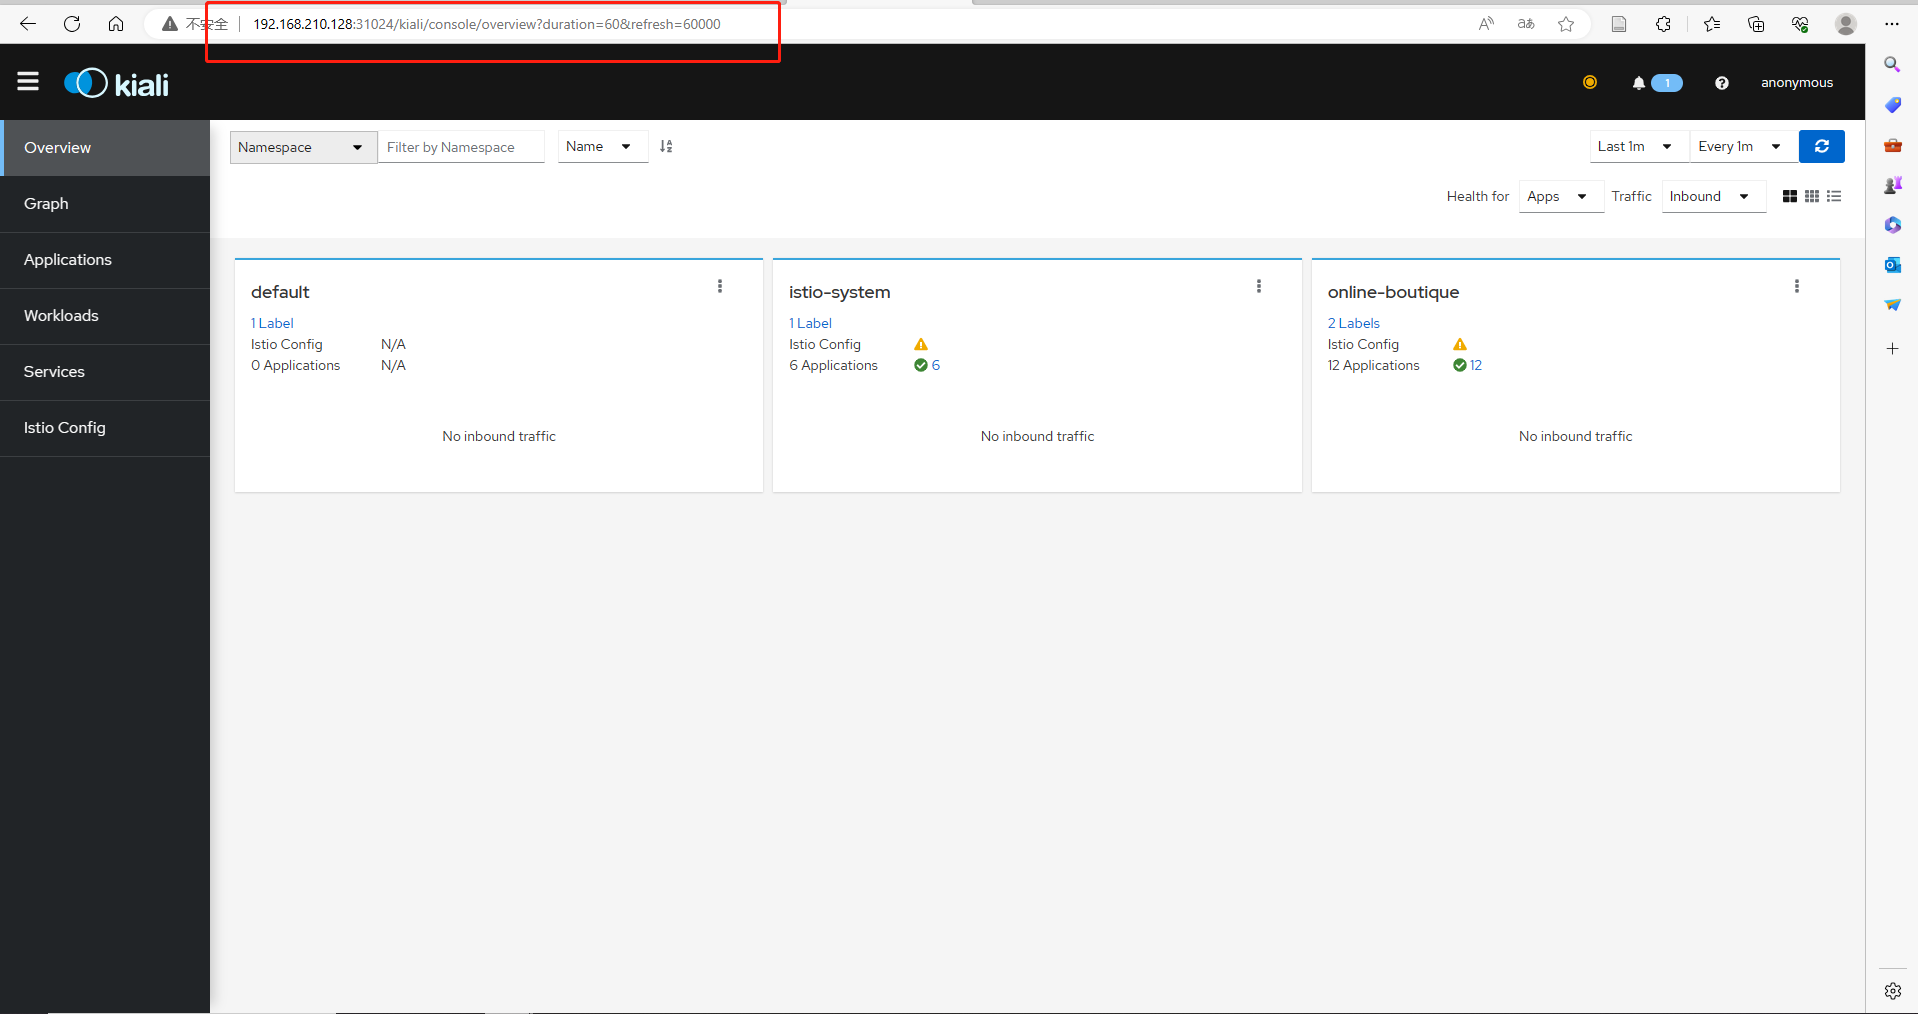
\includegraphics[width=1.0\textwidth]{figures/chapter3/kiali}
	\caption{Kiali首页}
	\label{fig:3-Kiali首页}
\end{figure}
Kiali提供了丰富的功能,使得服务网格的管理和可观察性更加便捷。
\begin{figure}[H]
	\centering
	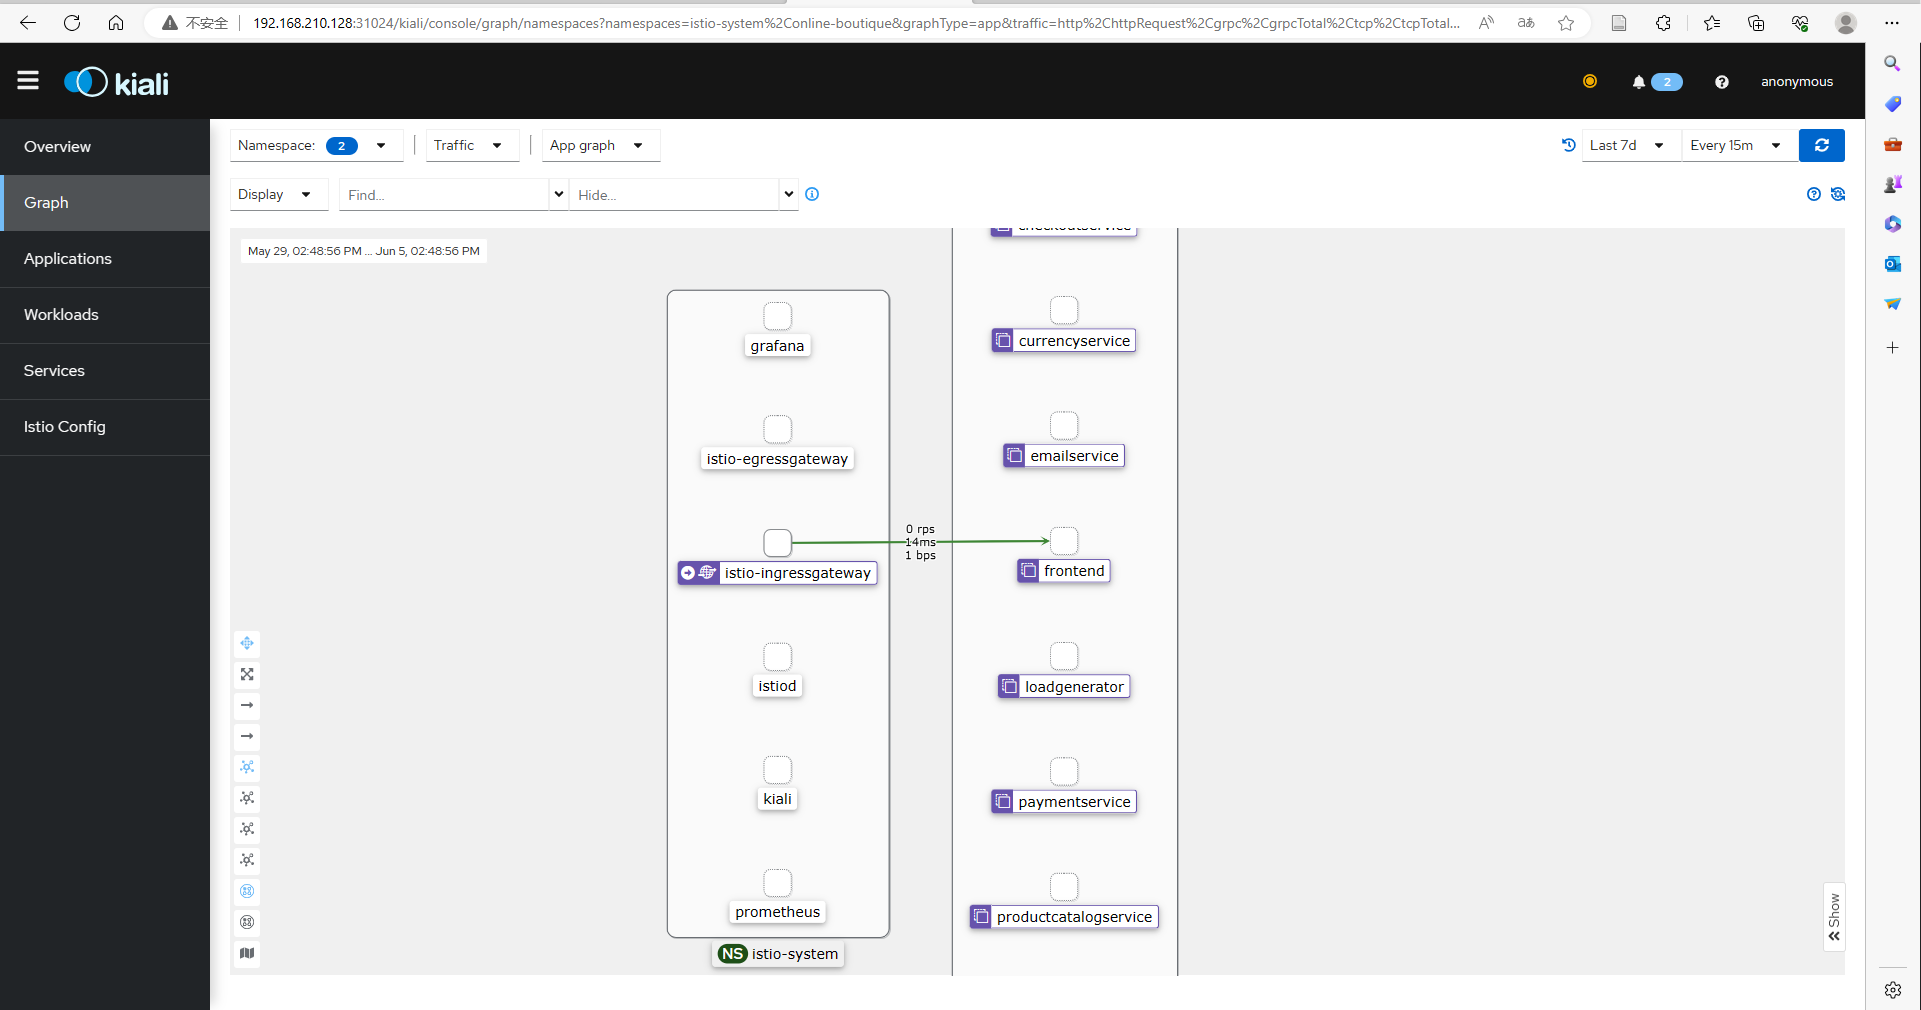
\includegraphics[width=1.0\textwidth]{figures/chapter3/online-boutique-kiali.png}
	\caption{Kiali服务拓扑图,以online-boutique为例}
	\label{fig:Kiali服务拓扑图,以online-boutique为例}
\end{figure}
Kiali生成一个服务拓扑图,展示了服务的拓扑结构,并将服务的通信方式可视化。图中的节点和边的颜色代表了服务网格的健康状况。红色或橙色的节点可能需要关注。节点的形状表示了组件的类型,如服务、工作负载或应用程序。该拓扑图还显示了入站和出站的指标,并提供与Jaeger和Grafana的集成,以便进行分布式追踪和性能监控。该图向我们展示了服务的拓扑结构,并将服务的通信方式可视化。它还显示了入站和出站的指标,以及通过连接 Jaeger 和 Grafana(如果安装了)的追踪。图中的颜色代表服务网格的健康状况。红色或橙色的节点可能需要注意。组件之间的边的颜色代表这些组件之间的请求的健康状况。节点形状表示组件的类型,如服务、工作负载或应用程序。
\begin{figure}[H]
	\centering
	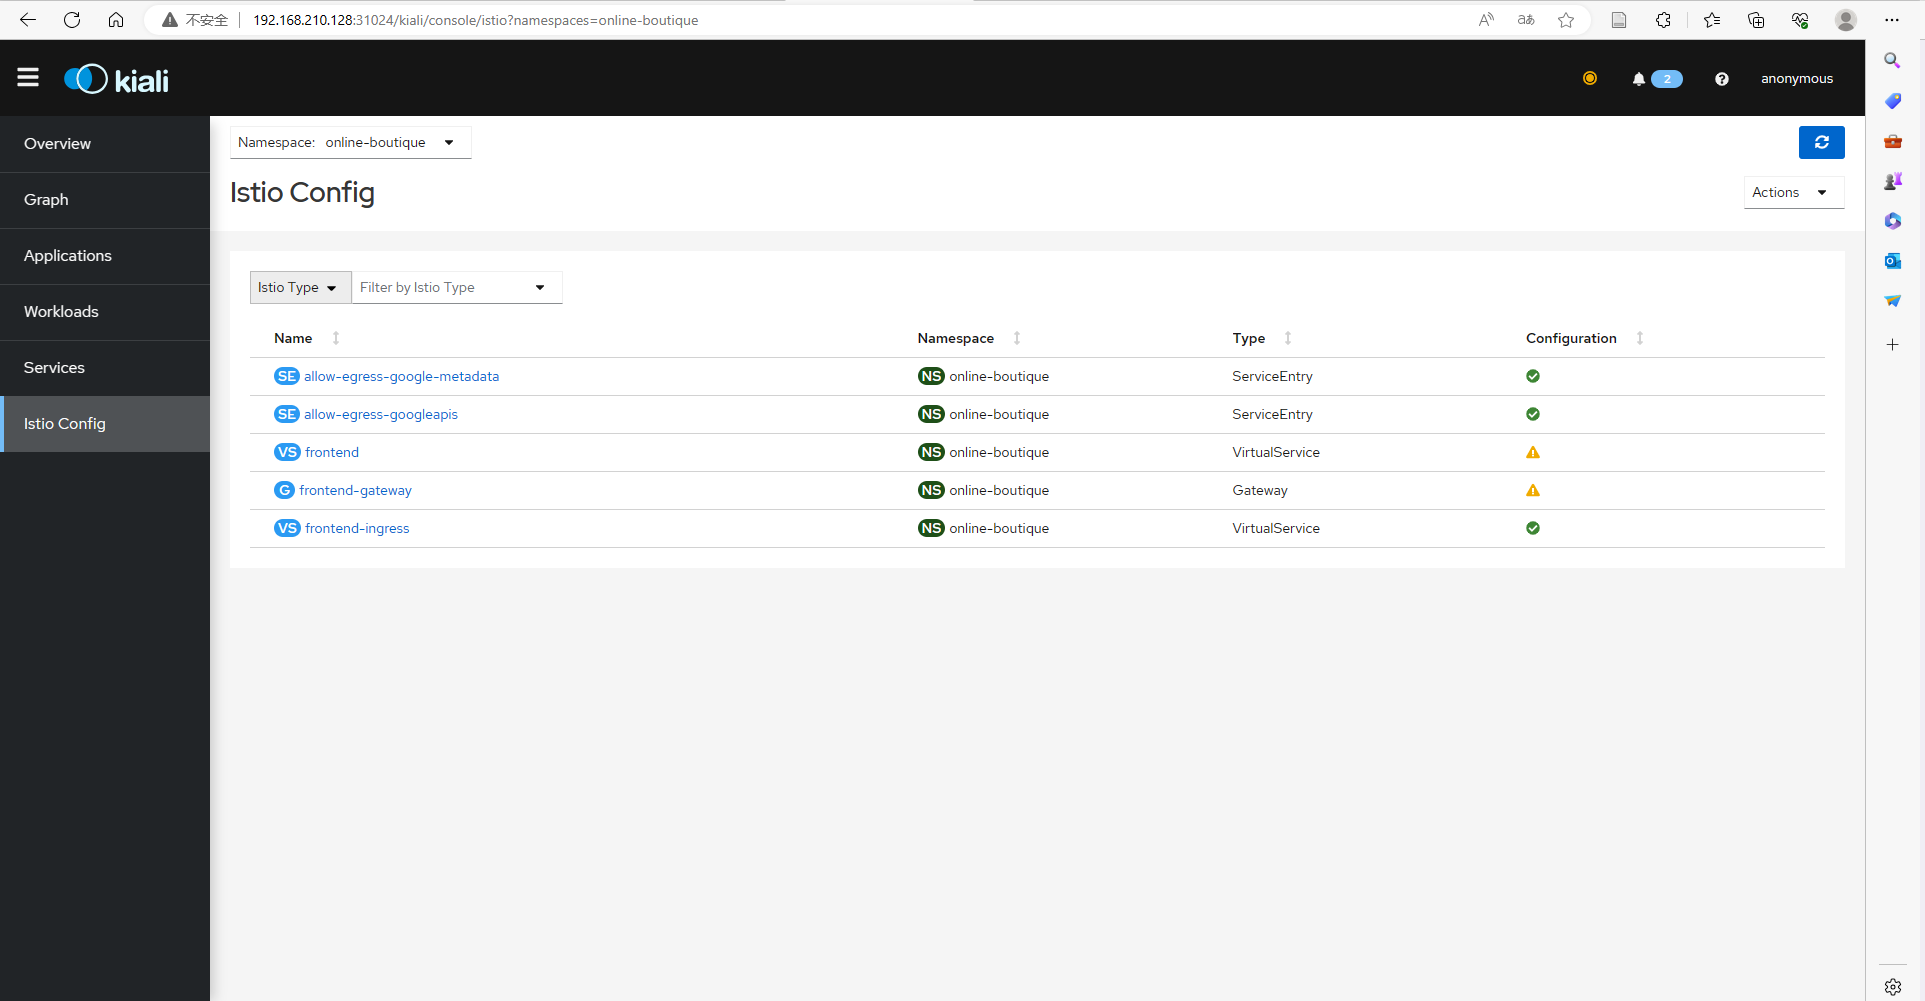
\includegraphics[width=1.0\textwidth]{figures/chapter3/kiali-config.png}
	\caption{Kiali创建、更新和删除Istio配置}
	\label{fig:3-Kiali创建、更新和删除Istio配置}
\end{figure}
Kiali允许通过向导驱动的方式创建、更新和删除Istio配置。用户可以通过Kiali界面配置请求路由、故障注入、流量转移和请求超时等功能。如果已经部署了现有的Istio配置,Kiali可以验证配置并报告任何警告或错误。Kiali的配置操作使得管理和调整服务网格变得更加直观和方便。通过Kiali,可以更好地管理和可视化服务网格,并进行配置和验证操作。同时,Kiali还提供了与Jaeger和Grafana等工具的集成,为分布式追踪和性能监控提供了便利。

\subsection{Jaeger 的配置与使用}
Jaeger是一个开源的分布式追踪系统,用于监控和故障排查分布式应用程序。它提供了端到端的追踪,使开发人员能够可视化请求在系统中的传播和处理路径,并识别潜在的性能瓶颈和故障点。

在分布式系统中,由于请求涉及多个服务和组件之间的相互作用,跟踪请求的流程和了解其在系统中的行为变得非常重要。Jaeger通过在分布式应用程序中插入轻量级追踪代码,收集跨服务边界的时间数据,以及请求在各个组件之间的传播路径和执行时间,从而提供了对应用程序性能和行为的深入洞察。

Jaeger提供了一个用户友好的界面,展示了请求的跟踪数据,包括请求的开始和结束时间、各个组件的处理时间、请求在组件之间的流转情况等。这些信息对于识别性能瓶颈、故障排查和系统优化非常有价值。

通过集成Jaeger客户端库和相关的追踪API,开发人员可以在他们的应用程序中生成和发送追踪数据给Jaeger进行分析。Jaeger提供了丰富的工具和API,以支持各种编程语言和框架,使开发人员能够轻松地将追踪功能集成到他们的应用程序中。

总而言之,Jaeger是一个强大的分布式追踪系统,为开发人员提供了对分布式应用程序的可观测性,帮助他们理解和优化应用程序的性能和行为。


使用jaeger.yaml文件安装Jaeger:
\begin{lstlisting}[language=bash]
	[root@k8scloude1 addons]# kubectl apply -f jaeger.yaml
\end{lstlisting}

安装完成后,可以使用以下命令检查Jaeger的部署情况:
\begin{lstlisting}[language=bash]
	[root@k8scloude1 addons]# kubectl get pod -n istio-system
\end{lstlisting}

默认情况下,Jaeger的Service类型为ClusterIP,无法从外部环境访问。为了让外部环境能够访问jaeger,需要将Jaeger的Service类型修改为NodePort。使用以下命令编辑Jaeger的Service:
\begin{lstlisting}[language=bash]
	[root@k8scloude1 addons]# kubectl edit service jaeger-collector -n istio-system
\end{lstlisting}

在打开的编辑器中,将Service的类型由ClusterIP修改为NodePort,并保存更改。之后可以使用以下命令获取Jaeger的Service信息:
\begin{lstlisting}[language=bash]
	[root@k8scloude1 addons]# kubectl get service -n istio-system
\end{lstlisting}

在输出中,可以看到Jaeger的NodePort端口号30038,可以在浏览器中访问Jaeger的网页界面。物理机IP地址为192.168.210.128,则可以在浏览器中输入以下地址:
\begin{lstlisting}[language=bash]
	http://192.168.210.128:30038
\end{lstlisting}
\chapter{使用Kiali进行流量路由追踪}
在本实验本实验旨在使用Kiali工具对流量路由进行追踪和监控,将使用Kiali进行流量路由追踪,以探索如何在Kubernetes环境中管理流量路由和版本控制。本实验将使用Istio作为服务网格,部署一个具有两个不同版本的前端服务,并使用Kiali来观察流量路由的变化。
\section{实验步骤}
\subsection{创建新的前端部署}
在开始实验之前,我们首先删除已经存在的前端部署。
\begin{lstlisting}[language=bash]
	kubectl delete deploy frontend
\end{lstlisting}
使用YAML文件创建一个新的前端部署,重新创建一个前端deploy,名字还是frontend,但是指定了一个版本标签设置为 original,修改后的yaml文件请见提交的代码。
创建deploy。
\begin{lstlisting}[language=bash]
[root@k8scloude1 ~]# kubectl apply -f frontend-original.yaml 
deployment.apps/frontend created
#deploy创建成功
[root@k8scloude1 ~]# kubectl get deploy | grep frontend
frontend                1/1     1            1           43s
#pod也正常运行
[root@k8scloude1 ~]# kubectl get pod | grep frontend
frontend-ff47c5568-qnzpt                 2/2     Running   0          105s
\end{lstlisting}
创建一个DestinationRule,用于定义两个前端服务的版本:原始版本(original)和新版本(v1)。创建frontend-dr.yaml ,在其中指定subsets,分别为orignal和v1,具体代码请见提交的代码文件。我们使用以下命令创建DestinationRule。
\begin{lstlisting}[language=bash]
	$ kubectl apply -f frontend-dr.yaml
\end{lstlisting}

\subsection{更新VirtualService}

接下来,使用以下命令更新VirtualService,并将所有流量路由到原始版本orginal的前端:
\begin{lstlisting}[language=bash]
kubectl apply -f frontend-vs.yaml
\end{lstlisting}

现在,我们准备创建新版本的前端部署。我们使用以下命令创建名为"frontend-v1"的部署:

\begin{lstlisting}[language=bash]
	$ kubectl apply -f frontend-v1.yaml
\end{lstlisting}

\subsection{更新流量路由权重}

最后,我们将更新VirtualService中的权重,将30%的流量路由到新版本的前端。我们使用以下命令更新VirtualService:

\begin{lstlisting}[language=bash]
	$ kubectl apply -f frontend-30.yaml
\end{lstlisting}
\section{实验结果}
我们通过浏览器访问INGRESS\_HOST,可以观察到前端界面的变化。在刷新页面的过程中,我们可以注意到来自新版本前端(v1)的更新标头和原始版本前端的标头之间的变化。

同时,我们可以使用Kiali工具查看服务的拓扑结构和流量路由。在Kiali界面中选择相应的命名空间和服务,我们可以观察到两个前端服务版本的运行状态以及流量的分布情况。

本实验通过使用Kiali工具对流量路由进行追踪和监控,展示了如何在服务网格中管理多个版本的服务,并灵活地进行流量分配和控制。通过使用Istio的DestinationRule和VirtualService功能,我们可以实现流量路由的精细控制,以满足不同的业务需求。

\chapter{使用Grafana监控故障注入}
本实验旨在使用Kiali工具对流量路由进行追踪和监控。我们将为推荐服务引入延迟和中止,然后使用Kiali和Grafana来观察流量路由和服务指标的变化。

首先,我们将为推荐服务引入5秒的延迟。我们创建一个名为recommendation-delay.yaml的YAML文件,并将以下内容保存到该文件中:

\begin{lstlisting}[language=bash]
apiVersion: networking.istio.io/v1alpha3
kind: VirtualService
metadata:
name: recommendationservice
spec:
hosts:
- recommendationservice.online-boutique.svc.cluster.local
http:
- route:
- destination:
host: recommendationservice.online-boutique.svc.cluster.local
fault:
delay:
percentage:
value: 50
fixedDelay: 5s
\end{lstlisting}

然后,我们使用以下命令创建VirtualService:

\begin{lstlisting}[language=bash]
$ kubectl apply -f recommendation-delay.yaml
\end{lstlisting}

\subsection{观察推荐服务延迟}

我们可以在浏览器中打开INGRESS\_HOST(http://192.168.110.190/),然后点击其中一个产品,观察推荐服务的结果。在刷新页面的过程中,我们会注意到页面要么立即加载,要么有一个延迟加载的页面,这是由于我们注入了5秒的延迟。

同时,我们可以打开Grafana界面(http://192.168.110.130:31092/),选择Istio服务仪表板,然后在服务列表中选择recommendationservice,查看Client Request Duration图表,观察延迟的变化。

\subsection{引入产品目录服务中止}

接下来,我们将为产品目录服务引入一个中止。我们创建一个名为productcatalogservice-abort.yaml的YAML文件,并将以下内容保存到该文件中:

\begin{lstlisting}[language=bash]
apiVersion: networking.istio.io/v1alpha3
kind: VirtualService
metadata:
name: productcatalogservice
spec:
hosts:
- productcatalogservice.online-boutique.svc.cluster.local
http:
- route:
- destination:
host: productcatalogservice.online-boutique.svc.cluster.local
fault:
abort:
percentage:
value: 50
httpStatus: 500
\end{lstlisting}

然后,我们使用以下命令创建VirtualService:

\begin{lstlisting}[language=bash]
$ kubectl apply -f productcatalogservice-abort.yaml
\end{lstlisting}

\subsection{观察产品目录服务中止}

如果我们刷新几次产品页面,我们应该会得到错误信息,指示产品目录服务中止。我们可以在Grafana界面查看报告的错误,并进一步分析流量路由和服务指标的变化。

\subsection{清理}

最后,我们可以使用以下命令删除创建的VirtualService:

\begin{lstlisting}[language=bash]
$ kubectl delete virtualservice recommendationservice
$ kubectl delete virtualservice productcatalogservice
\end{lstlisting}

\section{实验结果}

通过使用Kiali和Grafana,我们成功地观察到了推荐服务延迟和产品目录服务中止的效果。这些工具提供了对流量路由和服务指标的可视化和监控,有助于我们管理和调试服务网格中的流量分发。

\section{结论}

本实验展示了如何使用Kiali进行流量路由追踪,并结合Grafana进行服务指标的观察。通过注入延迟和中止,我们可以模拟不同的服务行为,并通过Kiali和Grafana来监控和分析流量路由和服务指标的变化。这些工具对于服务网格的管理和故障排除非常有帮助。

\chapter{引用与链接}\label{cha:ref}
\section{技术平台的底层实现机制}

\subsection{Kiali}

Kiali是一个用于观察和可视化服务网格的开源工具。它提供了对服务之间的通信、流量路由和服务指标的实时监控和可视化。Kiali的底层实现机制主要包括以下几个方面:

\begin{itemize}
	\item 与服务网格集成:Kiali可以与流行的服务网格平台(如Istio、Linkerd)进行集成,通过与网格控制平面通信来获取服务和路由的信息。
	\item 数据收集和存储:Kiali通过轮询网格控制平面或订阅其事件流来获取有关服务、路由和指标的信息。这些数据通常存储在Kiali自己的数据库中,以供查询和可视化使用。
	\item 可视化和监控:Kiali提供了一个用户界面,通过图表和图形展示服务之间的通信和流量路由。它还能够显示服务指标和性能数据,帮助用户监控和调试服务网格的行为。
	\item 配置和操作:Kiali允许用户对服务网格进行配置和操作,例如设置流量路由规则、注入故障和修改服务配置。这些操作通常通过Kiali的用户界面或API进行。
\end{itemize}

\subsection{Grafana}

Grafana是一个开源的数据可视化和监控平台,广泛用于展示和分析各种数据源的指标和日志。在服务网格中,Grafana通常与Prometheus等指标收集工具集成,用于可视化服务的性能和指标数据。其底层实现机制包括:

\begin{itemize}
	\item 数据源集成:Grafana可以与多种数据源进行集成,包括Prometheus、InfluxDB、Elasticsearch等。通过配置数据源连接,Grafana可以从这些数据源中获取指标和日志数据。
	\item 可视化和仪表板:Grafana提供了一个灵活的仪表板编辑器,用户可以使用图表、图形和面板来可视化数据。用户可以根据需求自定义仪表板的布局和样式,以便更好地展示和分析数据。
	\item 警报和通知:Grafana允许用户设置警报规则,当指标数据满足特定条件时触发警报。它还可以与各种通知渠道(如电子邮件、Slack)集成,及时通知用户关于警报事件的发生。
	\item 插件和扩展性:Grafana具有丰富的插件生态系统,用户可以安装和使用各种插件来扩展其功能。这些插件包括数据源插件、面板插件和应用插件,使用户能够根据需求进行定制和扩展。
\end{itemize}

\section{Online Boutique项目中的配置和使用步骤}

在Online Boutique项目中,Kiali和Grafana可以与Istio一起使用,以提供对服务网格的可视化和监控。以下是它们在项目中的配置和使用步骤:

\subsection{Kiali的配置和使用}

要在Online Boutique项目中使用Kiali,可以按照以下步骤进行配置和使用:

\begin{enumerate}
	\item 安装和配置Istio:首先,需要安装和配置Istio服务网格。可以按照Istio的官方文档进行操作,包括安装Istio控制平面和注入Istio代理(Envoy)到服务中。
	\item 安装Kiali:接下来,需要安装Kiali。可以从Kiali的官方网站下载适合您环境的Kiali版本,并按照其文档中的说明进行安装和配置。
	\item 连接到服务网格:配置Kiali以连接到已部署的服务网格。这通常涉及指定Istio控制平面的地址和凭据,以便Kiali可以获取有关服务和路由的信息。
	\item 访问Kiali界面:完成配置后,可以通过浏览器访问Kiali的用户界面。在界面中,您可以查看服务之间的通信和流量路由,查看服务指标和性能数据,并进行配置和操作,例如设置流量路由规则和注入故障。
\end{enumerate}

\subsection{Grafana的配置和使用}

要在Online Boutique项目中使用Grafana,可以按照以下步骤进行配置和使用:

\begin{enumerate}
	\item 安装和配置Prometheus:首先,需要安装和配置Prometheus作为数据源。可以按照Prometheus的官方文档进行操作,包括安装Prometheus服务器和配置指标收集目标。
	\item 安装Grafana:接下来,需要安装Grafana。可以从Grafana的官方网站下载适合您环境的Grafana版本,并按照其文档中的说明进行安装和配置。
	\item 配置Prometheus数据源:在Grafana中配置Prometheus作为数据源。这涉及指定Prometheus服务器的地址和凭据,以便Grafana可以从Prometheus中获取指标数据。
	\item 创建仪表板:使用Grafana的仪表板编辑器创建仪表板,以可视化服务的性能和指标数据。您可以选择不同类型的图表和面板,并根据需要进行配置和调整。
	\item 设置警报规则(可选):如果需要设置警报规则,可以在Grafana中配置警报规则,并指定触发警报的条件和通知渠道。这样,在特定条件满足时,Grafana将发送通知以提醒用户。
\end{enumerate}

通过以上步骤,您可以成功配置和使用Kiali和Grafana,以实现对Online Boutique项目的服务网格可视化和监控。您可以根据需要在Kiali和Grafana中进行进一步的配置和操作,以满足项目的需求。
\chapter{其它格式}
\section{代码}
\subsection{原始代码}
朴实的代码块:

使用 verbatim 环境可以得到如下原样的输出。
\begin{verbatim}
print("Hello world!")
\end{verbatim}

使用 listings 包提供的 lstlisting 环境可以对代码进行进一步的格式化,minted 包所提供的 minted 环境还可以对代码进行高亮。更多定制功能请自行参照文档配置。

\begin{lstlisting}[language=c, caption=C语言代码]
    printf("Hello world!");
\end{lstlisting}

\subsection{算法描述/伪代码}
参考 \href{https://en.wikibooks.org/wiki/LaTeX/Algorithms}{Algorithms} 与 algorithm2e 文档,给出一个简单的示例,见算法 \ref{alg:alg1}。

\begin{algorithm}[H]
  \SetAlgoLined
  \KwData{this text}
  \KwResult{how to write algorithm with \LaTeXe}
  initialization\;
  \While{not at end of this document}{
    read current\;
    \eIf{understand}{
      go to next section\;
      current section becomes this one\;
    }{
      go back to the beginning of current section\;
    }
  }
  \caption{如何写算法}\label{alg:alg1}
\end{algorithm}

\section{绘图}
关于使用 \LaTeX{} 绘图的更多例子,请参考 \href{https://www.overleaf.com/learn/latex/Pgfplots_package}{Pgfplots package}。一般建议使用如 Photoshop、PowerPoint 等制图,再转换成 PDF 等格式插入。

\section{写在最后}
工具不重要,对工具的合理运用才重要。希望本模板对大家的论文写作有所帮助。



%此处结束正文-------------------------------------------------------------------------------------------------


% !Mode:: "TeX:UTF-8"
%%%%%%%%%%%%%%%%%%%%%%%%%%%%-------结论--------%%%%%%%%%%%%%%%%%%%%%%%%%%%%%%%%

\acknowledgement
\addcontentsline{toc}{chapter}{结论}
%\linespread{1.5}

这里写本次实验的结论。

% 这里写本次实验的结论
















 %%%结论

%%%============================================================================================================%%%

%%%=== 参考文献 ========%%%
\cleardoublepage\phantomsection

\bibliographystyle{gbt7714-numerical}        % 参考文献样式,  plain,unsrt,alpha,abbrv,chinesebst 等等
\bibliography{ref/refs.bib}



%%%-------------- 附录. 不需要可以删除.-----------


\appendix

\chapter{测试}

\section{第一个测试}
测试公式编号
\begin{equation}
1+1=2.
\end{equation}

表格编号测试

\begin{table}[h]
  \centering
  \caption{测试表格}
  \begin{tabular}{*{20}c}
     \hline
     % after \\: \hline or \cline{col1-col2} \cline{col3-col4} ...
     11 & 13  & 13  & 13  & 13 \\
     12 & 14  & 13  & 13  & 13 \\
     \hline
   \end{tabular}
\end{table}
\chapter{附录测试}

%%%-------------- 教师评语评分 ------------------
\begin{teacher}
\thispagestyle{empty}
评语: 
\par
\vspace*{12.5cm}
\hspace*{7.5cm}评分: 
\vspace*{1cm}

\hspace*{7.3cm}评阅人:

\vspace*{0.5cm}

\hspace*{10.1cm}年\hspace*{1cm}月\hspace*{1cm}日

\vspace*{0.5cm}

{\songti \zihao{4} \makebox[1cm][s]{(备注:对该实验报告给予优点和不足的评价,并给出百分制评分。)}}

\end{teacher}


\cleardoublepage
\end{document}





